\documentclass[12pt]{article}
\usepackage{graphicx}
\graphicspath{ {images/} }
\usepackage[letterpaper, portrait, lmargin=1.5in, rmargin=1.25in, tmargin=1in, bmargin=1in]{geometry}
\usepackage{color}
\usepackage{setspace}
\usepackage{pdfpages}
\usepackage{booktabs}
\usepackage{dcolumn}
\newcounter{mysubtable}
\usepackage{amsmath}
\newcommand\modcounter{%
  \refstepcounter{mysubtable}%
  \renewcommand{\thetable}{\thesection.\arabic{table}\alph{mysubtable}}%
}

\makeatletter
%% The "\@seccntformat" command is an auxiliary command
%% (see pp. 26f. of 'The LaTeX Companion,' 2nd. ed.)
\def\@seccntformat#1{\@ifundefined{#1@cntformat}%
   {\csname the#1\endcsname\quad}  % default
   {\csname #1@cntformat\endcsname}% enable individual control
}
\let\oldappendix\appendix %% save current definition of \appendix
\renewcommand\appendix{%
    \oldappendix
    \newcommand{\section@cntformat}{\appendixname~\thesection\quad}
}
\makeatother

    \usepackage{tabularx}
\usepackage{adjustbox}
\usepackage{subcaption}
\DeclareCaptionSubType*[Alph]{table}
\DeclareCaptionLabelFormat{mystyle}{Table~\bothIfFirst{#1}{ }#2}
\captionsetup[subtable]{labelformat=mystyle}
\usepackage[toc,page]{appendix}
\usepackage[flushleft]{threeparttable}


\doublespacing


\title{The External Validity of Experimental Social Preference Games}
\author{Sarah Xu}
\date{April 2018}

\begin{document}

\maketitle

\section{Introduction}

The standard economic model assumes individuals\rq \ actions are motivated purely by self-interest. However, from simple observation it is clear that people actually care about the well-being of others: people volunteer, people donate to causes, and social programs exist. If someone is not solely motivated by material self-interest but also cares about the material payoffs of others, we say that the person has social preferences. The last few decades have seen a strong increase of interest in this topic, with numerous research studies providing evidence of social preferences. Many papers have identified various aspects of social preferences such as altruism, social welfare, inequality aversion, and reciprocity (e.g., Charness and Rabin 2000; Fehr and Schmidt 1999; Andreoni and Miller 2002; Rabin 1993; Fisman, Jakiela, and Kariv 2014). 
 
When studying social preferences, the typical approach is to conduct experiments in a laboratory setting. Participants play experimental games, where they receive monetary incentives aligned with the payoffs of the games. Researchers are able to control and influence prices, information, and actions available to the participants, which allows researchers to rigorously target different aspects of social behavior. Below are common games used to study social preferences, along with their typical social preference interpretations: 

\begin{itemize}

\item{Dictator Game}: The player (dictator) receives an endowment, \textit{m}. The dictator chooses how to split the amount between themselves and a second player (the receiver) so that \(\pi_{s} + \pi_{o} = \textit{m}\), where \(\pi_{s}\) is how much is kept and \(\pi_{o}\) is how much is given.
\subitem The dictator\rq s action is usually explained by concepts of altruism or fairness preferences (e.g. inequality aversion).
\item{Ultimatum Game}: Two-player game where two players bargain over a fixed endowment, \textit{m}. The first mover (proposer) divides the sum, so that \(\pi_{s} + \pi_{o} = m\). The second mover (responder) chooses to either accept or reject the offer. If accepted, the proposal is implemented. If rejected, neither player receives any money.
\subitem The proposer\rq s behavior is typically corresponded with fairness, and the responder\rq s response can be explained by negative reciprocity or fairness preferences such as inequality aversion.
\item{Trust Game}: Two-player game where the first player receives an endowment, \textit{m}, and proposes how to divide the endowment between themselves and the second mover so that \(\pi_{s} + \pi_{o} = m\). The second player (the responder) receives \(k\pi_{o}\), where k $>$ 1, and decides how much of the endowment to return to the first mover. 
\subitem The proposer\rq s action indicates their trust levels, and the responder\rq s return indicates their trustworthiness or reciprocity.
\item{Public Goods Game}: N-player game where each player receives the same sum of money, \textit{m}, and simultaneously decides how much to put into a public fund. The payoff function is given by \( P_{i} = m - g_{i} + \beta \sum_{n=1}^{N} g_{j} \) , where \(g_{i}\) is the amount that player \textit{i} donated to the fund, \(\beta\) is the marginal payoff of the public fund (0$<$\(\beta\)$<$N\(\beta\)), and \(\sum_{n=1}^{N}g_{j}\) is the sum of the individual donations to the public fund.
\subitem The players\rq actions are usually explained by their altruism, cooperation, or trust levels.
\end{itemize}

There is an abundance of literature that study social preferences using the mentioned experimental games (along with other papers using games not mentioned). For example, Forsythe (1994) recruited undergraduate students from the University of Iowa, where they played single dictator and ultimatum games against anonymous opponents. The authors found that, contrary to the subgame perfect Nash equilibrium that both proposers and responders would not send any money, most players in fact gave away proportions of the endowment given to them. Bert et al (1995) recruited undergraduate students from the University of Minnesota to participate in trust games. 94\% of the proposers sent money, and over one-third of the responders returned an amount greater than what was given to them, showing evidence of trust and reciprocity. Hermann, Thoni, and Gachter (2008) conducted public goods experiments across 16 participant pools, and found that that opportunities for punishment led to varying cooperation levels. used public goods game to provide evidence of punishment and reciprocity. These papers are only a few examples from an abundance of literature (with many papers using social preference games not mentioned above), making it clear that these games has become one of the building blocks of experimental and behavioral economics. 
 
However, laboratory experiments have a disadvantage: they are abstract and remote from realistic situations. Therefore, an important question is the extent to which the experimental games approach to social preferences can be generalized to real world situations. Human behavior may be influenced by a variety of factors that differ between practical and laboratory settings. One issue is that in a laboratory setting, the subject's actions are under the scrutiny of the researcher. Hoffman et al (1994) found that almost 50\% of their subjects donated at least \$3 (out of a \$10 pie) when playing the dictator game. However, when the authors implemented a ``double-blind'' treatment where both the experimenter and other subjects could not observe the dictator\rq s actions, they found that only 16\% of subjects gave at least \$3. There are other papers that also find that subjects are more prosocial in the lab than they are in the field (e.g., List, 2006; Gneezy et al., 2004). Individuals are also influenced heavily on the context of the situation. For example, in a two-person trust game, Burnham, McCabe, and Smith (2000) switched between calling the responder "partner" and "opponent", and found a significant difference in trust and trustworthy behavior. Similarly, Ross and Ward (1996) found that simply calling a prisoner's dilemma game either a ``community'' or ``Wall Street'' game wildly varied each treatment group\rq s rates of defection. There are also other studies that find that slightly changing the narrative could result in significant changes in behavior (e.g., Andreoni 1995; Gintis 2001;  Henrich et al 2005). Studies also find evidence that varying the level of stakes may lead to significantly different behaviors. For example, Carpenter, Verhoogen, and Burks (2005) find that increasing the stakes from \$10 to \$100 decreased the median offer in the dictator game from 40\% to 20\%. Slonim and Roth (1998) and Parco, Rapoport, and Stein (2002) also find that higher stakes leads to significantly different results than with lower stakes. Interestingly, however, Cherry, Frykblom, and Shogren (2002) find no differences in offers when increasing the stakes from \$10 to \$40. Of course, scrutiny, context, and stakes are only a few factors that can lead to deviations in behavior\footnote{see Levitt and List (2007) for a full discussion of factors, with supporting literature, that can lead to deviations in behavior between laboratory and field settings.}.
 
The fact that varying factors such as scrutiny, context, and stakes can yield significant differences in behavior calls into question the external validity of using experimental games in a laboratory setting to study social preferences. There are a few studies that have examined how subjects\rq \ behavior in a lab setting is compared to the same subjects\rq  behavior in a real world situation, and found that in-lab behavior does predict field behavior. Baran et al (2010) compared MBA alumni donations to their university with their reciprocity behavior when playing the trust game. The authors find that responder behavior predicted university donations. Franzen and Pointner (2013) compared behaviors from university students participating in standard dictator games to their actions when receiving a misdirected letter containing money, and found that subjects who showed prosocial behavior in the lab returned the misdirected letters more often than subjects who were selfish in the lab. Englmaier and Gebhardt (2010) conducted field experiments where they compared university students\rq free riding behavior at the library with free riding behavior in a public goods game, and found statistically significant correlation between field and lab measures. There are also a couple studies that used non-student subjects: Fehr and Leibbrandt (2011) conducted public goods games with Brazilian fishermen, and found that fishermen who are more cooperative in the games were also less likely to exploit the communal fishing grounds. Karlan (2005) compared Peru inhabitants\rq \ trust game behavior to their micro loans repayment behavior, and found correlation between behaviors in the lab game and in the field. 

On the other hand, there are a number of papers that find lab behavior has no predictive power for field behavior. Goeschl et al (2015) examined university students\rq \ behavior in two different tasks: a public goods game and their contributions to a task about reducing CO2 emissions. The authors find that behavior in both tasks is uncorrelated. Hill and Gurven (2004) carried out ultimatum and public goods games on Paraguay Ache Indians. They compared the behaviors to observed food production and sharing patterns to individuals outside the nuclear family and found no significant relationships to lab behavior. Gurven and Winking (2008) recruited Tsimane forager-horticulturalists in Bolivia, and compared behavior when playing dictator and ultimatum games to their food-sharing behavior. The authors find no relation between the two measures. Voors et al (2012) studied farmers in Sierra Leone, and compared their behavior in a public goods game to their behavior when asked to contribute to a real community public good. They find no meaningful correlation in behavior between the lab and field measures. 

With other studies finding statistically significant, not statistically significant, and mixed results, the currently accumulated evidence is ambiguous. Galizzi and Navarro-Martinez (2017) summarize that about 40\% of reported lab-field correlations and regressions found statistically significant association between lab and field behaviors\footnote{see Galizzi and Navarro-Martinez (2017) for their full systematic review and meta-analysis of literature on within-subjects lab-field studies}. It is clear that evidence for the external validity of experimental games is weak, justifying that further research is needed. Galizzi and Navarro-Martinez (2017) note, however, that the previous studies compare only one social preference game to one specific field measure. The abstract and context-free nature of the games makes it difficult to theoretically map the game to the field measure, and so it is crucial to have a more systematic approach. The authors proceed to carry out their own study where participants answered questions about social behaviors exhibited in the past, played various social preference games, and encountered naturalistic field situations. The field situations included a research assistant asking for help carrying boxes down the stairs, asking to use the participant\rq s phone to make a brief phone call, asking for donations to a children\rq s charity, asking for donations to an environmental charity, or asking for donations to the lab\rq s research fund.  The authors\rq \ overarching conclusion is that behavior when playing the experimental games does a poor job predicting both the survey questions and the field behaviors. They do mention, however, that more systematic studies are needed to draw a definite conclusion.

It is critical to think about why some studies found correlations between lab and field measures and some studies did not, in order to inform the design of my current experiment. While playing the experimental games for Hill and Gurven (2004)\rq s study, participants expressed worry that their choices would make the receiver upset. In particular, the tribal group\rq s culture was heavily focused on community, and was well known for extensive food sharing (which was the field measure the authors used). Perhaps the participants didn\rq t want to risk their choices creating any tension in their community, and getting punished with less food sharing and cooperation. For the last two papers, the stakes were a result of high scrutiny and low anonymity since it was easy for community members to find out the choices each subject made. For my design, an important aspect is that participants will play the games in their own time and location to ensure no scrutiny and high anonymity.

Adopting Galizzi and Navarro-Martinez (2017)\rq s design, I will recruit Wesleyan University seniors and recent alumni to play various experimental games.  The different social preference games include the generalized dictator game, ultimatum game, trust game, and public goods game. I will further describe each game, as well as their relevance to my chosen field measure, in the next section.

A criticism of Galizzi and Navarro-Martinez\rq s design is how the authors executed their field measures: since the setups occur as the participants are exiting their lab session, it is hard to believe that the participants did not connect the encounters to the research lab, especially since they previously answered questions similar to the current event. This may have led to actions that participants would not have done if they were unaware of the scrutiny. Therefore it is better to use a natural, far-removed situation. For my study, I will use Wesleyan University donations as the field measure. Further discussion on my choice of field measure is in the next section.

Similar to previous lab-field experiments, I will examine whether in-lab social behavior predicts real-life social behavior. In addition, along with playing various experimental games, participants will answer non-incentivized questions regarding their past social behavior. I will use the self-reported measures as an additional layer to evaluate the explanatory ability of the games. By comparing my results with those of past lab-field studies, I can contribute to the discussion on whether experimental games are a useful tool to examine social preferences

{\color{red} BRIEF OVERVIEW OF RESULTS .. IS IT IN LINE WITH GALIZZI/NAVARRO PAPER? THEY FOUND POOR JOB. }

The rest of the paper is organized as follows: Section 2 describes the methods used; Section 3 presents the results obtained; and Section 4 discusses the results.


\section{Methods}

Each participant was presented with two sets of tasks: (i) incentivized social preference games, and (ii) survey questions regarding past social behavior. The field measure used to compare to participants\rq \ lab results is their Wesleyan University donations. The goal of this design is to evaluate the external validity of experimental social preference games to behaviors in the field. In addition, I will examine whether another tool (self-reported measures) or both tools can better predict social preferences exhibited in real-world situations. 
 
Wesleyan University seniors and recent alumni received an invitation email briefly explaining my research and asking for participation in my study (emails were provided by Wesleyan University Relations). The entire study was computerized, programmed and implemented using Qualtrics. Online links to both the experimental games and survey questions were included in the email, so those who chose to take part could complete the study remotely. As mentioned in the previous section, the online structure allows participants to make decisions anonymously and without scrutiny, minimizing the risk for exaggerated behavior. Participants received an overview of the two tasks they would complete, and were informed that upon completion of the study, their major, class year, and Wesleyan donations information would be released to me.

In order to incentivize completion of both the games and survey questions, as well as elicit honest game behavior, participants were also informed that completing the entire study made them eligible for a lottery prize. All games used "tickets" as the experimental currency unit: the total tickets each person earns directly corresponds with how many lottery tickets they own.

I will now explain each of the three main components.

\subsection{Incentivized social preference games}

Those who chose to participate in the study received a unique identifier assigned to them by Qualtrics. Participants first played four social preference games: generalized dictator game, ultimatum game, trust game, and public goods game. Before each game, they received detailed instructions along with an example to illustrate how each game worked. For the ultimatum and trust games, each participant will have the opportunity to play the roles of both proposer and responder.

Below are the games each participant played: 

\begin{itemize}

\item{Generalized Dictator Game (GDG)}:  Each participant plays as the dictator (Player 1). They are asked to make a series of choices on how to divide tickets between themselves and an anonymous, random Player 2. Every ticket that Player 1 earns will be worth 1, 2, 3 or 4 tickets, depending on the choice. Similarly for the earnings of Player 2. Based off of Andreoni and Miller (2002)'s design, there will be nine rounds (in random order) with varying prices and endowments.
\item{Ultimatum Game}: 
	\begin{itemize}
		\item{Player 1 (UG1)}: Each participant plays as the proposer (Player 1), and is endowed with 10 tickets. They decide how much of their endowment to send to an anonymous, random responder (Player 2). They are told that the responder may or may not reject the allocation. If the allocation is rejected, neither player receives any tickets in this round.
		\item{Player 2 (UG2)}: Each participant is now the responder. They are given a list from 0 tickets to 10 tickets (in 1-ticket increments), and are asked whether they accept or reject for each listed amount.
	\end{itemize}
\item{Trust Game}:
	\begin{itemize}
		\item{Player 1 (TG1)}: Each participant plays as the proposer, and is endowed with 10 tickets. They decide how much of their endowment to send to an anonymous, random responder. The amount sent over is multiplied by three. The responder then decides how many tickets to return. 
		\item{Player 2 (TG2)}: Now each participant is the responder. They receive a list of all ten possible multiplied amounts that the proposer could have chosen to send. For each amount, they are prompted to enter the number of tickets they would like to return back to the proposer.
	\end{itemize}
\item{Public Goods Game (PGG)}: Each participant is endowed with 10 tickets and decide how much of their endowment to contribute to a group fund with one other anonymous, random participant. The total tickets in the group fund is multiplied by 2 and divided evenly between the two players.

\end{itemize}

Appendix A contains all materials - images of each game, along with their respective instructions and examples - from the online study.

At the end of the participation deadline, all participants were randomly paired, and ticket payoffs were calculated.

\subsubsection{Strategy Method}

Since the participants are completing the games at their own availability, they were not randomly matched with other participants until after all data had been collected. As seen with the ultimatum and trust games, which required both a proposer and responder, the responder saw a list of all possible offer amounts and was prompted for their choice for each offer. This is called the strategy method.

There are several reasons why the strategy method is advantageous. It is useful to have all of the responder\rq s potential choices so that payoffs can be determined. Most importantly, the strategy method gives more information. If players were matched with other players live, then we would only have the responder\rq s response given the proposer\rq s offer. The strategy method, however, provides all returned amounts for all possible donated amounts in the ultimatum game, and provides participants\rq \ minimum accepted amount. 

\subsubsection{Payment}

Participants were randomly paired, and ticket payoffs were determined for each game. In each assigned pair, one participant was randomly selected to be Player 1 (i.e. they were the dictator in the generalized dictator game, and proposer in both the ultimatum game and trust game), and the other was Player 2 (i.e. they were the receiver in the generalized dictator game, and the responder in both the ultimatum and trust game). I ran through each game and calculated ticket payoffs for each participant. Since the generalized dictator game consisted of nine rounds, one round was randomly selected. and each participant received the tickets based on their decision for that round. However many total tickets each participant earned from all the games corresponded with the number of tickets they owned in the lottery. Ten tickets were drawn, and each winner received \$100. Winners were emailed instructions on how to receive the prize through direct deposit.

\subsection{Self-reported measures of past social behaviors}

Participants then reported on social behaviors exhibited in the past. The questions are adapted from the Self-Report Altruism (SRA) scale introduced by Rushton, Chrisjohn, and Fekken (1981). The survey is comprised of 10 items, and participants report how frequently they have done each item in the past. Participants rate each statement as either ``Never'', ``Once'', ``More than once'', ``Often'', or ``Very often''. Examples include: ``I have donated money at the cash register when buying groceries'', ``I have pointed out a clerk\rq s error (at the supermarket, at a restaurant) in undercharging me'', and ``I have donated instead of sold my clothes/used items''. A full list of the 10 items from the online study is displayed in Appendix B. 

\subsection{Field Measure}

After the participation deadline passed, Wesleyan University Relations provided a dataset that contained each participant\rq s Wesleyan donations information.

Seniors are solicited around once per semester, during senior events. Recent alumni are typically solicited for donations at the end of November / beginning of December, March, and June. Since my online study was released between solicitation cycles for both seniors and recent alumni, and donations information was provided as of January 2018, donations are independent of my study. 

There are several reasons why I chose to use donations as my field measure. First, many behavioral economics papers exploring the relationship between in-lab and field behavior have used donations (e.g. Falk, Meier, and Zehnder 2011; Benz and Meier 2008; Baran et al 2010). Falk, Meier, and Zehder (2011) say they chose to use donations because {\color{blue}``First, the measure does not rely on self-reported survey responses but on actual decisions. Second, donation decisions are made in private and never made public. Third, students are unaware that their behavior is analyzed in a research study. Fourth, and most importantly, all students at the university have to decide about the donations.''}

Another reason is that donations may represent various social preference constructs. The most common representation is altruism, but donating can represent other concepts such as reciprocity, cooperation, and trust. In the context of using Wesleyan University donations, donating may represent reciprocity and trustworthiness since seniors/recent alumni may donate as thanks for providing them four years of education and opportunities. Donating may also represent trust since donors are trusting that the University will putting their donations to good use, and cooperation because the University solicits for donations. {\color{blue} Donating may also symbolize fairness preferences, more specifically inequality aversion: donors are able to target what area their donations can go towards. For example, if the donor targets their donations to Financial Aid, then they are displaying inequality averse preferences.}

Finally, donations is a more accurate field measure than creating a scenario at the end of the online session. Wesleyan donations is a far-removed situation, and is not directly related to the study. I previously mentioned that Galizzi and Navarro-Martinez (2017)\rq s design is unsatisfactory since their subjects encountered the field experiment shortly after completing the lab experiments, and reasoned that it would not be difficult for participants to link the two situations together. If I were to create a field situation at the end of the lab session, participants may feel compelled to act more pro-socially than they normally are since they know their actions are being scrutinized. In my design, participants\rq \ donations behavior is not affected by their participation in the lab.

\subsubsection{Theoretical Correspondences Between Games and Donations}

All the games I chose for my study tap into the different types of pro-social behaviors related to donating discussed in the previous section. First, the GDG and PGG responses are typically interpreted as altruism preferences. GDG, UG1, UG2, and PGG actions typically indicate fairness preferences. Lastly, TG1 represents participants\rq \ trust levels, and TG2 represents participants\rq trustworthiness and reciprocity. Therefore, each game can be theoretically mapped to donations behavior.
	
\subsection{Participants and Sessions}

Wesleyan University Relations provided a random sample of 2004 emails (334 emails for each class year from 2013 to 2018), and I sent an invitation email in early January 2018 asking for participation in my study. Participants were informed that the study consisted of several experimental games and non-incentivized survey questions, and participation should take no more than 15 minutes.  The deadline for participation was mid-February 2018. A total of 397 people completed the online study. The participants were volunteers who opened the Qualtrics link, provided consent for me to receive their major, class year, and Wesleyan donations data, and completed both the survey questions and social preference games. At the end of the participation deadline, all participants were randomly paired, ticket payoffs were calculated, and 10 winners were randomly selected. The winners were emailed  in the begging of March 2018 with instructions on how to receive their prizes.

\section{Results}
The results are presented in four distinct sections. I first start by briefly describing the results obtained in the three main elements (social preference games, self-report measure of past social behaviors, and donations). The fourth section will focus on the main research question of the paper: the extent to which the games explain the field behavior. Appendix C contains the variables definition table, and Appendix D contains all of the figures, correlation tables, and regression tables from this section.

\subsection{Social Preference Games}
Since the GDG consisted of 9 rounds with varying sets of endowments and prices of giving, similar to Andreoni and Miller (2002) and Fisman, Kariv, and Markovits (2007), I assume each participant\rq s giving preferences is a member of the constant elasticity of substitution (CES) utility function.  The CES utility function is written as: \\

\(U_{s} = [\alpha(\pi_{s})^{\rho} + (1-\alpha)(\pi_{o})^{\rho}]^{1/\rho} \) \\

\noindent
where \(\alpha\) measures the relative weight on the payoff for self, \(\rho\) indicates the willingness to trade off payoffs to self and other in response to price changes, and \(\sigma = 1/(\rho - 1) \) is the elasticity of substitution. Maximizing utility subject to the budget constraint ( \(p_{s}\pi_{s} + p_{o}\pi_{o}=m\) ) yields the CES demand function given by: \\
 
\(\pi_{s}(p,m)=\frac{[\alpha/(1-\alpha)]^{1/(1-\rho)}}{\rho^{-\rho/(\rho-1)}+[\alpha/(1-\alpha)]^{(1/(1-\rho)}}m\) \\

\hspace{15mm} \(= \frac{A}{p^{r}+A}m \) \\
 
 \noindent
where \(r=-\rho / (1-\rho) \) and \(A=[\alpha / (1-\alpha)]^{1/(1-\rho)} \). This generates the following individual-level econometric specification for each participant \textit{i}: \\
 
\( \pi^{t}_{s,i} = \frac{A_{i}}{(p^{t}_{i})^{r_{i}} + A_{i}}m^{t}_{i} + \epsilon^{t}_{i}\) \\
 
\noindent
where \textit{i} represents each participant, \textit{t} represents each independent decision-problems in the GDG, and \( \epsilon^{t}_{i} \) is assumed to be distributed normally with mean zero and variance \(\sigma^{2}_{i}\). For each participant \textit{i}, I used the 9 combinations of \(\pi_{s}\), p, and \textit{m} and generated the estimates \( \hat{A}_{i} \)and \( \hat{r}_{i} \) using non-linear least squares. From the estimates I retrieved each participant\rq s efficiency level, \( \hat{\rho_{i}}\), which then gave me each participant\rq s sharing propensity, \( \hat{\alpha_{i}} \).

Results for TG1, UG1, and PGG are represented by the proposer\rq s pass rates (the percentage of the initial endowment passed to the other player or public pool). UG2 is represented by the minimum pass rate the responder chooses to accept. 

TG2 asks for the participant\rq s return amount given the 10 possible offer amounts from Player 1 in TG1. For each participant, I regressed their return amount on the offer amount, and retrieved the estimated slope. The estimated slope represents the participant\rq s reciprocity, or trustworthiness level. Values closer to 1 represent more reciprocal behavior, and lower levels closer to 0 represent more selfish behavior. There may be concern that some participant\rq s may not follow a linear trend. After plotting each participant\rq s return amount in response to the offer amount, I found that with the exception of a few participants, each participant\rq s data points follow a linear slope.

Figure 1 consists of 2 panels (Panels A and B) that shows the distribution of parameters, \(\alpha\) and \(\rho\), derived from responses in GDG.  The parameter estimates vary dramatically across subjects, implying that preferences for giving are very heterogeneous. Panel A displays a high peak of 21\% at \(\alpha\)=1: a considerable amount of participants displayed extremely selfish preferences. There is a smaller peak of 12\% at \(\alpha\)=0.5, and there are more \(\alpha\) levels above 0.5 than below 0.5. These results show that participants tended to have more selfish preferences. To facilitate presentation of Panel B, participants with very negative \(\rho\) values were combined into the leftmost bar. About 7\% of subjects have perfect substitutes preferences for giving (\(\rho \approx 1\)): these subjects prefer to give their entire endowment to Player 2 when the price of giving is less than one, and keep their entire endowment when the price of giving is greater than one, i.e. efficiency-minded preferences. A little over 20\% of participants demonstrated Leontief preferences (\(\rho\) far below 0), i.e. they prefer splitting the endowment equally, and roughly 15\% of subjects possess Cobb-Douglas preferences (\(\rho \approx 0\)). Many subjects also have intermediate values of \(\rho\): 24\% have preferences for increasing total payoffs (\(0.1 \leq \rho \leq 0.9\)), and almost 20\% have preferences for reducing differences in payoffs between self and others (\(-0.9 \leq \rho \leq 0.9\)).

Figure 2 consists of 4 panels (Panels C, D, E, and F) which shows the distribution of responses in UG1, UG2, TG1, and PGG, respectively. Panel C reports a high 42\% spike at giving half of their endowment to Player 2, and there is slightly more emphasis on giving contributions lower than half the endowment than contributions higher than half the endowment. These results are in line with the typical patterns in previous literature, which finds that a majority of offers are in the range of 25?50\%. Correspondingly, Panel D shows the distribution of the minimum offers that Player 2 chooses to accept in UG2. With the exception of 1 participant who showed extreme negative reciprocity by only accepting an offer of Player 1's entire endowment, everyone accepted an amount less than or equal to half of Player 1's endowment. Surprisingly, most participants (27\%) accepted an offer amount of 0 tickets. Panel E shows contributions scattered all across the range from offering 0\% to 100\% of their given endowment in TG1 with two spikes, both around 22\%, at giving half the endowment or the entire endowment. Other contributions that have more than 10\% participants are giving 30\% or 40\% of the given endowment. This is also broadly in line with typical findings that report average transfers of roughly 50\% of endowment. Panel F shows that almost half the participants in PGG send their entire endowment into the public pool. The next most popular choice (20\%) is to send half their endowment to the public pool, and only 4\% of participants sent 0\% into the public pool. Again, this broadly matches usual results in literature.

Figure 3 contains 2 panels (Panels G and H) that displays the distribution of reciprocity levels and average repayment rate, respectively, which are derived from participants\rq \ responses in TG2. Panel G shows that, with the exception of two participants who demonstrated negative reciprocity (perhaps they did not understand the game), reciprocity levels are very heterogenous between 0 and 100. There is a spike (27\%) at reciprocity levels around 0.5, and a lower spike (14\%) around 0.35. There is also a small spike (10\%) at 0, which represents those who did not show any reciprocity. Panel H shows a strong peak of repayment rates of around 45\%, with participants showing slightly stronger preference repaying less than half of what was received versus repaying more than half of what was received. These results are in line with typical patterns found in previous literature, which report average repayment rates of nearly 50\% of the transfer.

Table 1 shows the pairwise correlations (Spearman\rq s \(\rho\)) between the different game outcomes. A large majority of the correlations are statistically significant at the 5\% level (12 out of 15). All of the statistically significant negative correlations involve the \(\alpha\) levels from GDG and the behavior in UG2. The negative correlations for \(\alpha\) reflect that participants who are more selfish (\(\alpha \rightarrow 1\)) are more likely to make smaller contributions in the other games, and the negative correlations for UG2 reflect that participants who accept smaller contributions are more likely to make larger contributions in the other game decisions. Otherwise, decisions in UG1, TG1, TG2, and PGG have positive correlations with one another.
These results show that participants demonstrated consistent behavior in all the games.

\subsection{Self-Reported Measures of Past Social Behaviors}

SRA scores are obtained by summing across each participant\rq s responses for the 10 items in the SRA Scale (``Never'' = 0, ``Once'' = 1, ``More than once'' = 2, ``Often'' = 3, ``Very often'' = 4). A higher SRA score indicates higher pro-social behavior. Figure 4 shows the distribution of total scores. There was a wide variety in the total SRA scores obtained, ranging between 20 and 48. Scores are centered around 33 and the shape is symmetric. Panel J displays the distribution of SRA scores including only the items related to money (items 2, 3, 4, and 7). A large majority of the scores are between 9 and 12.

Table 2 contains pairwise correlations (Spearman\rq s \(\rho\)) between the game responses and the SRA scores. I included both total SRA scores (``SRA'') and monetary SRA scores (``SRAmoney''). None of the game results are significantly correlated with total SRA scores, and only two games, TG2 and PGG, are significantly correlated with the monetary SRA scores. Overall, there is a very weak relationship between the social preference games and self-reported measures. 

\subsection{Donations Behavior}

Figure 5 shows the distribution of Wesleyan donations. Panel I shows that 64\% of the participants have donated to Wesleyan University before, and 36\% have not. Panel J shows the distribution of total donation amounts below \$100, with donations above \$100 aggregated into the rightmost bar. Most of the donation amounts are below \$20 (about 36\%). There are 30 participants who have donated a total amount greater than \$100. All of these donations amounts are between \$100 and \$625, with the exception of two very large donations.

\subsection{External Validity of Social Preference Games}
I now turn to the main question of whether the game decisions explain the field behavior. There are two ways that I represented the field measure: (1) whether the participant has donated or not, and (2) the total amount the participant has donated. First, Table 3 presents ten logistic regression models, using the binary donations representation as the response variable. The first eight columns present each of the games, total SRA results, and monetary SRA results on their own. The last two columns includes all of the game results along with the total and monetary SRA scores, respectively. None of the games or SRA results are statistically significant on their own. In addition, when both the games and SRA results are used in the regression model, neither of the variables are statistically significant. I then regressed the same explanatory variables on the amount donated. As shown in Figure 5, most donations amounts were fairly small. I therefore used two-limit tobit maximum likelihood, setting the restriction that 0 $\leq$ donations $\leq$ 50.  Table 4 presents the eight tobit models. The total SRA variable is statistically significant at the 10\% level and the monetary SRA variable is statistically significant at the 5\% level, while none of the social preference games results are statistically significant.

It is also useful to look at the R$^{2}$ values, which measures the proportions of variance explained by the regressors. For both the logistic and tobit regressions, I calculated each models\rq \ McFadden\rq s pseudo-R$^{2}$ values. The values are shown at the bottom of each table. Table 3 shows all of the models have very low values - practically zero - with the highest belonging to the model that includes both the games and monetary SRA score. Table 4 also reports pseudo-R$^{2}$ values that are very low, and again, the highest value belongs to the model that includes both the games and monetary SRA score. 

Tables 3 and 4 provide evidence that the social preference games, even when combined with self-reported measures, have little to no power to explain donations behavior. However, this may be because the right combination of variables are not included in the models. I performed best subset selection on both the logistic and tobit regression models\footnote{Best subset selection identifies all of the possible regression models derived from all of the possible combinations of the candidate predictors, and determines the model that does the best at meeting some well-defined criteria. In this case, the criteria I used is Mallows\rq \ \(C_{p}\)-statistic, which assesses assess fits when models with different numbers of parameters are being compared.  See Mallows (1973).}. Since best subset selection fits all possible models to find the best candidate, I included more explanatory variables: I added the GDG parameter \(\rho\), the TG2 average return outcome, and replaced the total and monetary SRA scores with each of the ten individual SRA questions. I first performed best subsets regression for the logistic model, and four of the SRA items were chosen (items three, four, eight, and ten) . Table 5 displays the logistic regression model with those chosen variables. All of the chosen SRA items are statistically significant at the 5\% level. The pseudo-R$^{2}$ value of the model is a lot better than the previous logistic models in Table 3 (almost 8 times larger than the highest value), although it is still very high. I then ran best subsets selection for the tobit model, and only the \(\rho\) parameter was selected. Table 6 contains the tobit regression that includes only \(\rho\). However, the variable is still not statistically significant, and the psuedo-R$^{2}$ value is not better than the models in Table 4.

Overall, a few of the SRA items are a slightly better tool than both social preference games and total/monetary SRA scores to explain whether people donate or not, and \(\rho\) was chosen as the best variable to explain the amount people decide to donate. However, each models\rq \ chosen variables still explained little to none of the variability of donations behavior. While these results may be discouraging regarding the external validity of social preference games, this switches us to another interesting question: if these tools - experimental games and self-reported measures - do a poor job explaining donations behavior, can they still be a useful tool to predict donations behavior? If Wesleyan University wanted to predict which seniors or recent alumni will donate, or the amount donated, then perhaps using social preference games and/or SRA measures can help them target who to solicit donations from.

The least absolute shrinkage and selection operator (lasso) is a useful regression analysis method that performs both variable selection and regularization in order to enhance prediction accuracy\footnote{ 
the lasso estimate is defined by \\ \\
\( \beta^{lasso}=\mathop\mathrm{argmin}\limits_{\beta} \{ \frac{1}{2} \sum_{i=1}^{N} (y_{i} - \beta_{0} - \sum_{j=1}^{p}x_{ij}\beta _{j})^{2}+\lambda\sum_{j=1}^{p}|\beta _{j}|\} \) \\ \\
where \(\lambda\) is a free parameter set to minimize the out of sample error. Certain coefficients are truncated to be set to zero to effectively choose a simpler model that does not include those coefficients. In other words, lasso regression works like a feature selector that picks out the most important coefficients, i.e. those that are most predictive (and have the lowest p-values). See Tibshirani (1996) for a full introduction on the lasso method.}.
I first used the lasso method on the logistic model, and all of the variables except for two of the SRA items were shrunk to zero. Table 7 reports the lasso penalized logistic model, where both SRA coefficients are statistically significant at the 5\% level\footnote{statistical significance tests were based off of Lockhart et al (2014)\rq s proposed significance test for the lasso. See Kyung et al (2010) and Tibshirani (1996) for a full discussion on standard errors for lasso predictions.}. I then used the lasso method on the continuous donations model, and found that all of the variables were truncated to zero. In summary, self-report measures were chosen to be better for predicting whether people will donate or not, and neither games nor self-report measures were good tools for predicting donation amounts.



\section{Discussion and Conclusion}

Thoughts:

self-report measures seem to be pretty much the same usefulness (if not better) than experimental games - chosen as in best subset selection, and chosen in lasso regression.

the self-report measures that were chosen were money-related. (But I only had 10 SRA items)
predict whther ppl donate or not, but not how much ppl will donate.

Potential policy implication with findings from a research perspective. Experimental games are costly - not only is it expensive paying participants for attending the lab session and providing money aligned with the payoffs of the games (especially if more show up than expected), but it also takes a lot of time to program the experimental games. If experimental games do not better predict field measures, then perhaps eliminate experimental games and instead using survey questions is better for funding and logistical purposes. 

however this is just the beginning of a systematic approach to uncovering the external validity of experimental social preference games. what can further research do?
population - other than university students (self-selected??)
use more far-removed, naturalistic field measures - i only 1 field behavior - may be difficult since alumni donations are recorded but other forms of charitable giving are not really

potentially spark interest into future studies into the external validity of other behavioral economics topics where lab experiments are also commonly used. For example, using experiments to study risk preferences and time preferences is common, so it will be interesting to see whether in-lab behavior is correlated to field measures, and perhaps adopting a systematic approach (comparing a variety of lab experiments to various field measures) can prove to be beneficial.


 \newpage
\begin{thebibliography}{9}

\bibitem{AndreoniMiller}
Andreoni, J., and Miller, J.H. (2002).
\textit{Giving according to GARP: An experimental test of the consistency of preferences for altruism}.
Econometrica, 70, 737-53.

\bibitem{Baran}
Baran, N.M., Sapienza, P., and Zingales, L. (2010).
\textit{Can we infer social preferences from the lab? Evidence from the trust game}.
NBER Working Paper 15654.

\bibitem{Benz}
Benz, M., and Meier, S. (2006).
\textit{Do people behave in experiments as in the field? Evidence from donations}.
Experimental Economics, 11, 268-81.

\bibitem{Berg}
Berg, J., Dickhaut, J.W., and McCabe, K.A. (1995).
\textit{Trust, reciprocity, and social history}.
Games and Economic Behavior, 90, 166-93.

\bibitem{Burnham}
Burnham, T., McCabe, K., Smith, V. (2000).
\textit{Friend-or-foe intentionality priming in an extensive form trust game}.
Journal of Economic Behavior \& Organization, 43, 57-73.

\bibitem{Carpenter}
Carpenter, J.P., Verhoogen, E., and Burks, S. (2005).
\textit{The effect of stakes in distribution experiments}.
Economics Letters, 86, 393-98.

\bibitem{CharnessRabin}
Charness, G., and Rabin, M. (2002).
\textit{Understanding social preferences with simple tests}.
Quarterly Journal of Economics, 117, 817-69.

\bibitem{Cherry}
Cherry, T., Fykblom, P., and Shogren, J. (2002).
\textit{Hardnose the Dictator}.
American Economic Review, 92(4): 1218-21.

\bibitem{Englmaier}
Englmaier, F., and Gebhardt, G. (2010)
\textit{Free-riding in the lab and in the field}.
CESifo Working Paper No. 3612.

\bibitem{FehrLeibbrandt}
Fehr, E., and Leibbrandt, A. (2011)
\textit{A field study on cooperativeness and impatience in the Tragedy of the Commons}.
Journal of Public Economics, 95, 1144-55.

\bibitem{FehrSchmidt}
Fehr, E., and Schmidt, K. (1999).
\textit{A theory of fairness, competition, and cooperation}.
Quarterly Journal of Economics, 114, 173-68.

\bibitem{Fisman1}
Fisman, R., Jakiela, P., and Kariv, S. (2014).
\textit{The distributional preferences of Americans}.
NBER Working Paper.

\bibitem{Fisman2}
Fisman, R., Kariv, S., and Markovits, D. (2007).
\textit{Individual Preferences for Giving}.
American Economic Review, 97(5): 1858-76.

\bibitem{Franzen}
Franzen, A., and Pointner, S. (2013)
\textit{The external validity of giving in the dictator game: A field experiment using the misdirected letter technique}.
Experimental Economics, 16, 155-69.

\bibitem{Galizzi}
Galizzi, M., and Navarro-Martinez, D. (2017).
\textit{On the external validity of social preference games: a systematic lab-field study}.
Management Science.

\bibitem{Gintis}
Gintis, H. (2000).
\textit{Strong reciprocity and human sociality}.
Journal of Theoretical Biology, 206, 169-79.

\bibitem{Gneezy}
Gneezy, U., Haruvy, E., and Yafe, H. (2004).
\textit{The inefficiency of splitting the bill: A lesson in institutional design}.
The Economic Journal, 114(495), 265-80.

\bibitem{Goeschl}
Goeschl, T., Kettner, S.E., Lohse, J., and Schwieren, C. (2015)
\textit{What do we learn from public good games about voluntary climate action? Evidence from an artefactual field experiment}.
University of Heidelberg, Department of Economics Discussion Paper 595.

\bibitem{GurvenWinking}
Gurven, M., Winking, J. (2008).
\textit{Collective action in action: prosocial behavior in and out of the laboratory}.
American Anthropologist, 110(2), 179-190. 


\bibitem{Henrich}
Henrich, J., et al. (2005).
\textit{``Economic Man'' in Cross-Cultural Perspective: Ethnography and Experiments from 15 Small-Scale Societies}.
Behavioral and Brain Sciences. 28(6): 795?815.

\bibitem{Hermann}
Hermann, B., Thoni, C., and Gachter, S. (2008).
\textit{Anti-social punishment across societies}.
Science, 319, 1362-67.

\bibitem{HillGurven}
Hill, K., and Gurven, M. (2004)
\textit{Economic experiments to examine fairness and cooperation among the Ache Indians of Paraguay}.
In J. Henrich, R. Boyd, S. Bowles, C. Camerer, E. Fehr, and H. Gintis (Eds.),
Foundations of Human Sociality: Economic Experiments and Ethnographic Evidence from Fifteen Small-Scale Societies. Oxford University Press.

\bibitem{Hoffman}
Hoffman, E., McCabe, K., Shachat, K., and Smith, V. (1994).
\textit{Preferences, property rights, and anonymity in bargaining games}.
Games and Economic Behavior, 7(3): 346-80.

\bibitem{Karlan}
Karlan, D.S. (2005).
\textit{Using experimental economics to measure social capital and predict financial decisions}.
American Economic Review, 95, 1688-99.

\bibitem{Levitt}
Levitt, S., and List, J. (2007)
\textit{What do laboratory experiments measuring social preferences reveal about the real world?}.
Journal of Economic Perspectives, 21(2), 153-74.


\bibitem{List}
List, John. 2006.
\textit{The behavioralist meets the market: measuring social preferences and reputation effects in actual transactions}.
Journal of Political Economy, 114(51), 1-37.


\bibitem{Parco}
Parco, J., Rapoport, A., and Stein, W. (2002).
\textit{Effects of financial incentives on the breakdown of mutual trust}.
Psychological Science.

\bibitem{Rabin}
Rabin, M. (1993).
\textit{Incorporating fairness into game theory and economics}.
The American Economic Review, 83, 1281-1302.

\bibitem{Ross}
Ross, L., and Ward, A. (1996).
\textit{Naive realism in everyday life: Implications for social conflict and misunderstanding}.
Values and Knowledge, 103-35.

\bibitem{Rushton}
Rushton, J.P., Chrisjohn, R.D., and Fekken, G.C. (1981).
\textit{The altruistic personality and the self-report altruism scale}.
Personality and Individual Differences, 2, 293-302.

\bibitem{Slonim}
Slonim, R., and Roth, A. (1998).
\textit{Learning in high stakes ultimatum games: An experiment in the Slovak Republic}.
Econometrica, 66, 569-96.


\bibitem{Voors}
Voors, M., Turley, T., Kontoleon, A., Bulte, E., and List, J.A. (2012).
\textit{Exploring whether behavior in context-free experiments is predictive of behavior in the field: Evidence from lab and field experiments in rural Sierra Leone}.
Economic Letters, 114, 308-311.


\end{thebibliography}

\newpage

\appendix
\section{Computerized Social Preference Games} \label{app:a} 
\vspace{8mm} 
\noindent Generalized Dictator Game (GDD) \\ \\
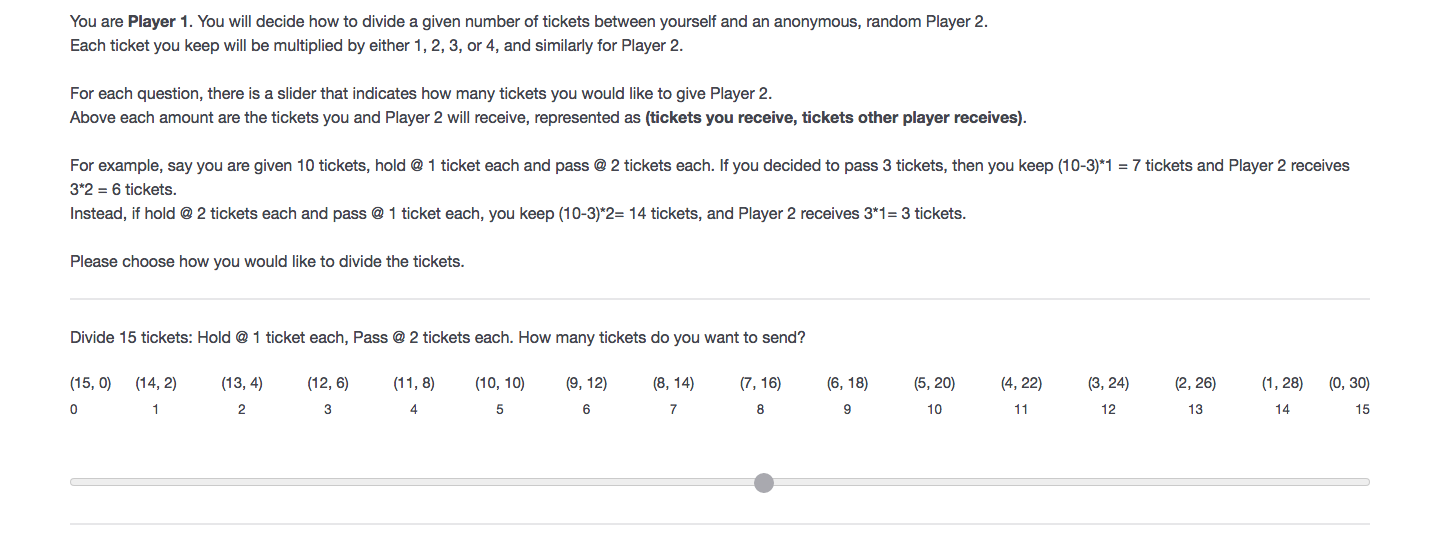
\includegraphics[scale=0.35]{gendict1}\\
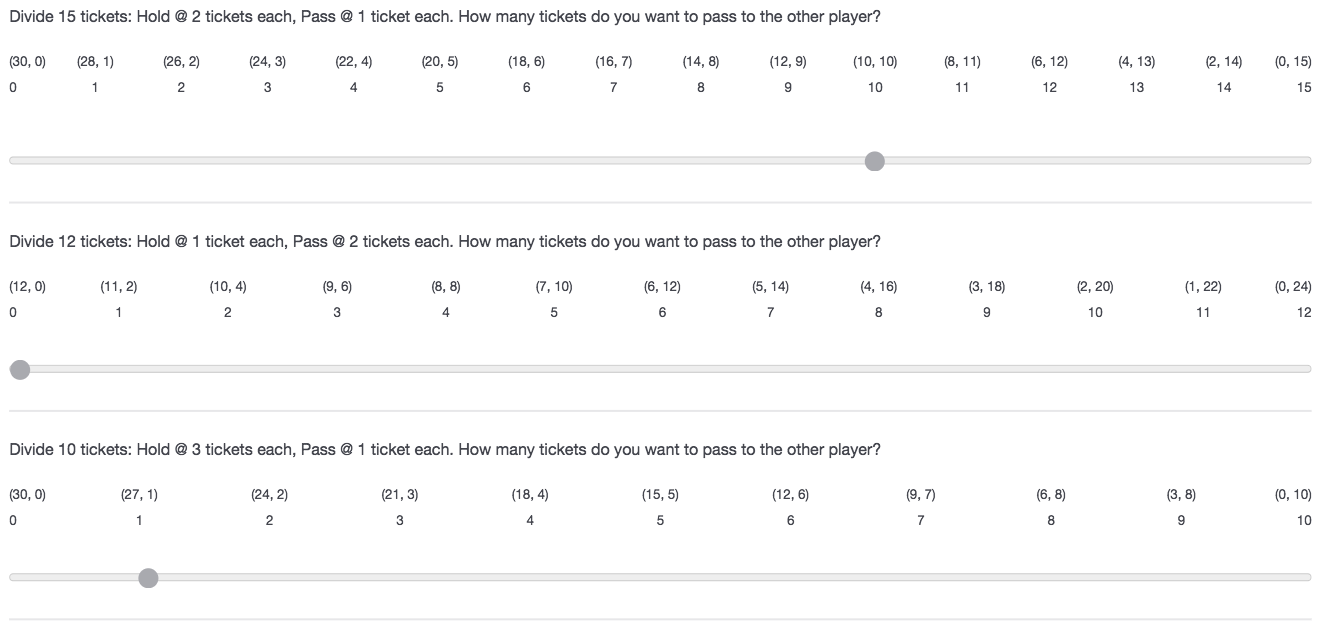
\includegraphics[scale=0.35]{gendict2}\\
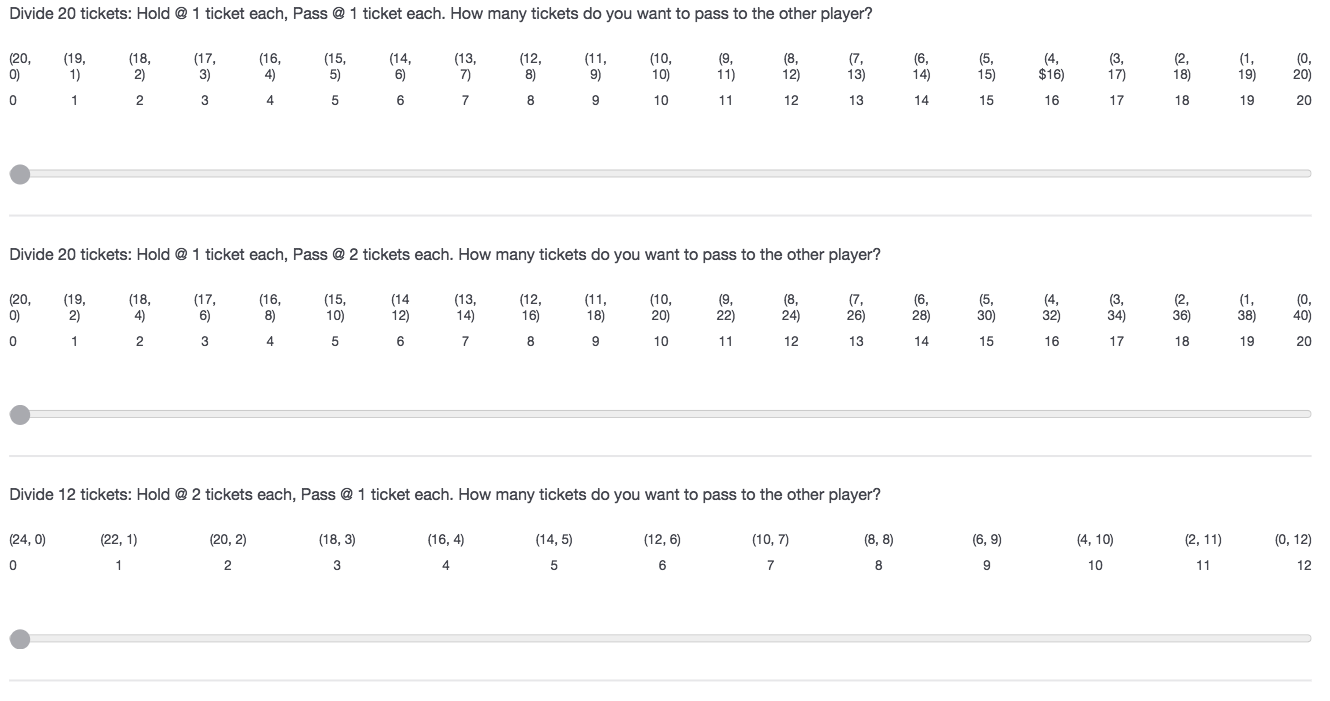
\includegraphics[scale=0.35]{gendict3}\\
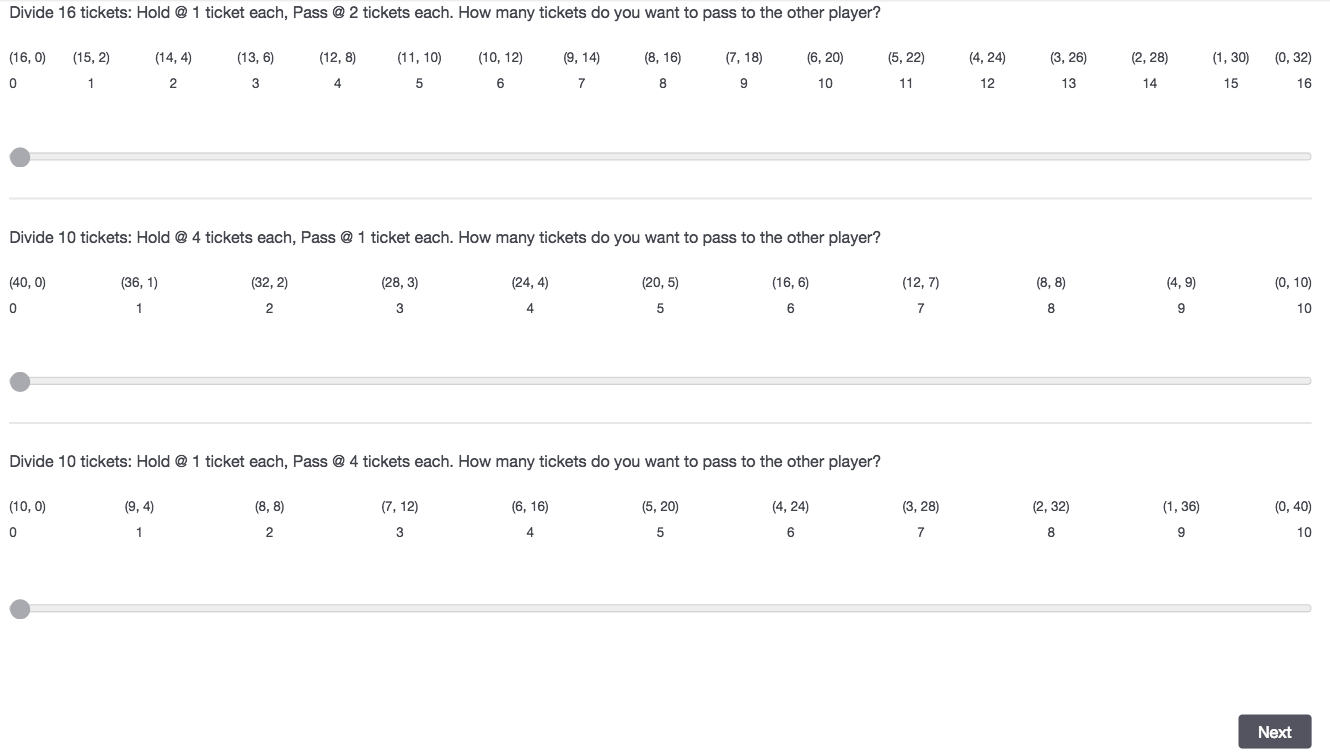
\includegraphics[scale=0.35]{gendict4}\\ \\
\noindent Ultimatum Game Player 1 (UG1) \\ \\ 
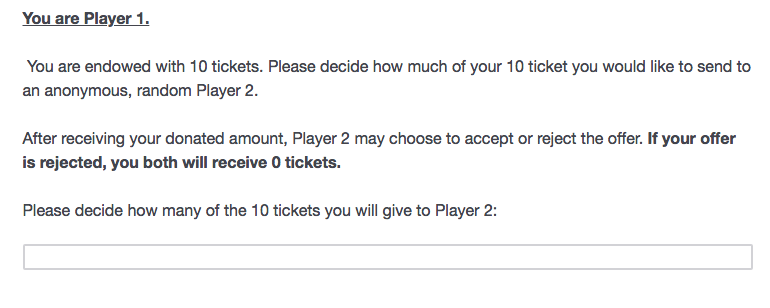
\includegraphics[scale=0.35]{ultimatum1} \\ \\
\noindent Ultimatum Game Player 2 (UG2) \\ \\
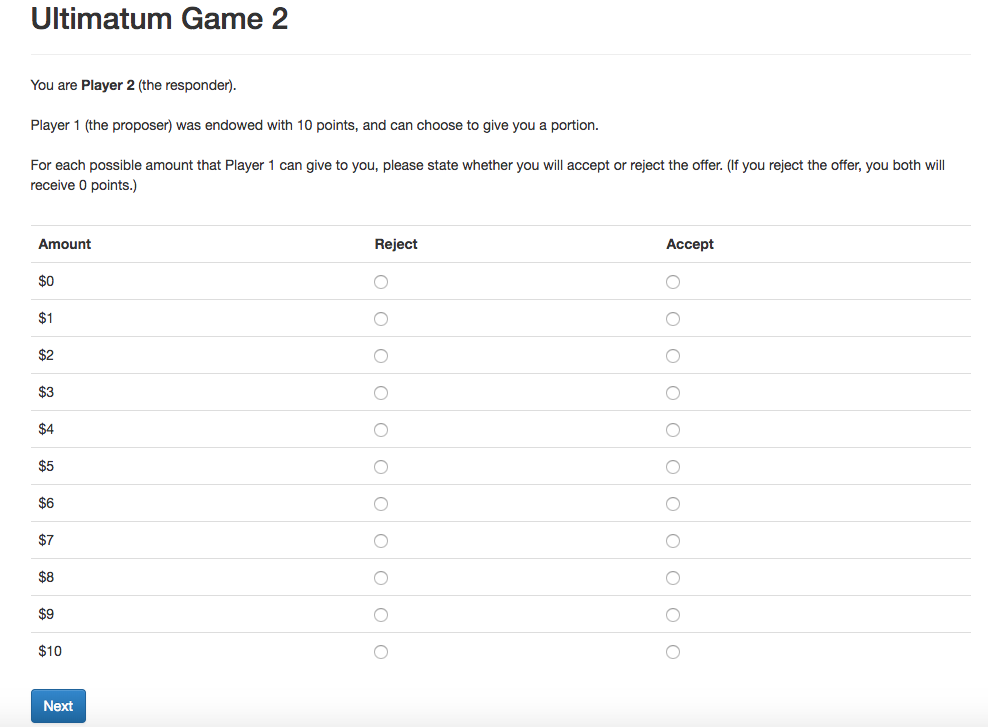
\includegraphics[scale=0.35]{ultimatum2} \\
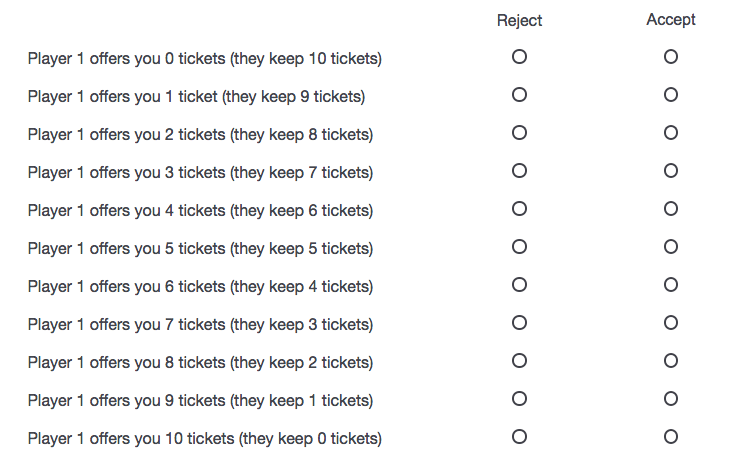
\includegraphics[scale=0.35]{ultimatum3} \\ \\
\noindent Trust Game Player 1 (TG1) \\ \\
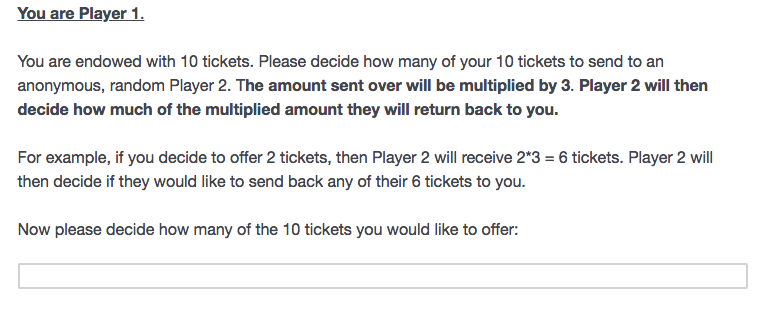
\includegraphics[scale=0.35]{trust1} \\ \\
\noindent Trust Game Player 2 (TG2) \\ \\
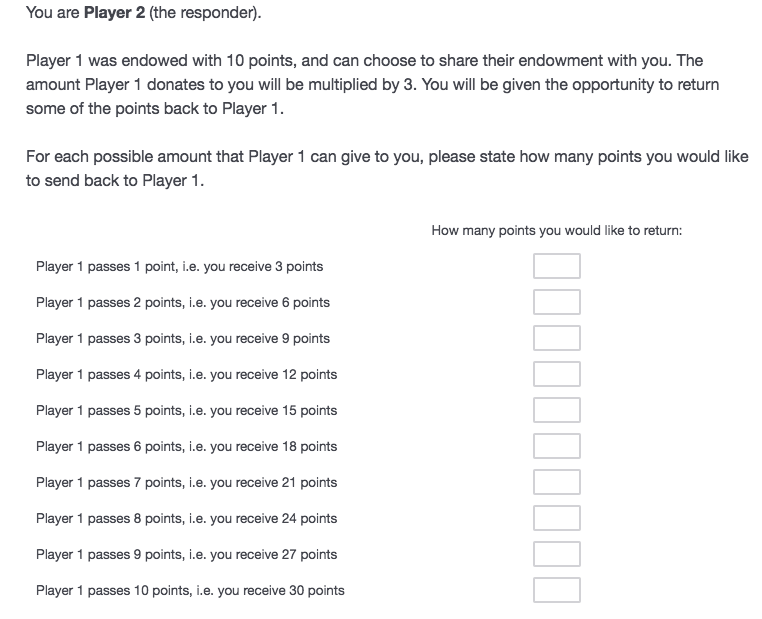
\includegraphics[scale=0.35]{trust2} \\
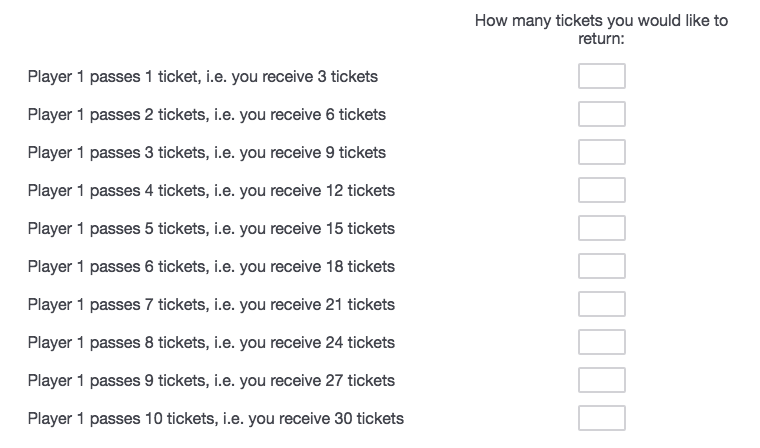
\includegraphics[scale=0.35]{trust3} \\ \\
\noindent Public Goods Game (PGG) \\ \\
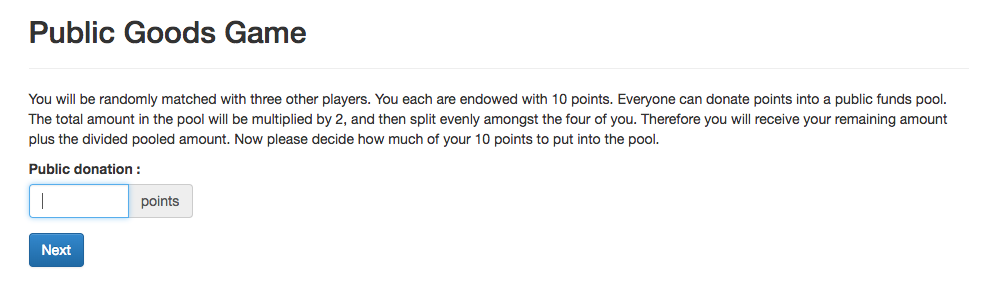
\includegraphics[scale=0.35]{public} \\


\section{Self-Report Altruism (SRA) Questions List} \label{app:b}


\begin{tabular}{ | p{12cm} | }
\hline
%\multicolumn{1}{|c|}{SRA Questions List} \\
%\hline
1. I have allowed someone to go ahead of me in line.\\
\hline
2. I have donated money at the cash register when buying groceries.\\
\hline
3. I have given money to a stranger (or an acquaintance I don\rq t know too well) in need.\\ 
\hline
4. I have donated to a charity.\\
\hline
5. I have done volunteer work for a charity/organization.\\
\hline
6. I have delayed an elevator/held door open for stranger(s).\\
\hline
7.  I have pointed out a clerk\rq s error (at a supermarket, restaurant) in undercharging me.\\
\hline
8. I have gone out of my way to meet with someone to help them with a task (e.g. help proofread their paper, listen to their presentation, etc). \\
\hline
9. I have offered my seat on a bus/train to a stranger who was standing.\\
\hline
10. I have helped an acquaintance with moving in/ moving out of their dorm/apartment/house.\\
\hline
\end{tabular} \\ \\ 

\section{Variables Definition Table} \label{app:c}

\begin{center}
\begin{tabular}{ |c|c| } 
 \hline
 Alpha & Player\rq s \(\alpha\) level derived from the generalized dictator game \\ 
 \hline
 UG1 & Player 1\rq s pass rate in ultimatum game \\ 
 \hline
 UG2 & Player 2\rq s minimum pass rate accepted in ultimatum game  \\ 
 \hline
 TG1 & Player 1\rq s pass rate in trust game \\ 
 \hline
 TG2 & Player 2\rq s reciprocity level in trust game \\ 
 \hline
 PGG & Player\rq s pass rate into public pool in public goods game  \\ 
 \hline
 SRAmoney & Player\rq s monetary SRA score \\ 
 \hline
 SRAtotal & Player\rq s total SRA score \\ 
\hline
\end{tabular}
\end{center}

\newpage


\section{Figures and Tables} \label{app:d}

\noindent Figure 1: Distribution of CES parameters from GDG \\ \\
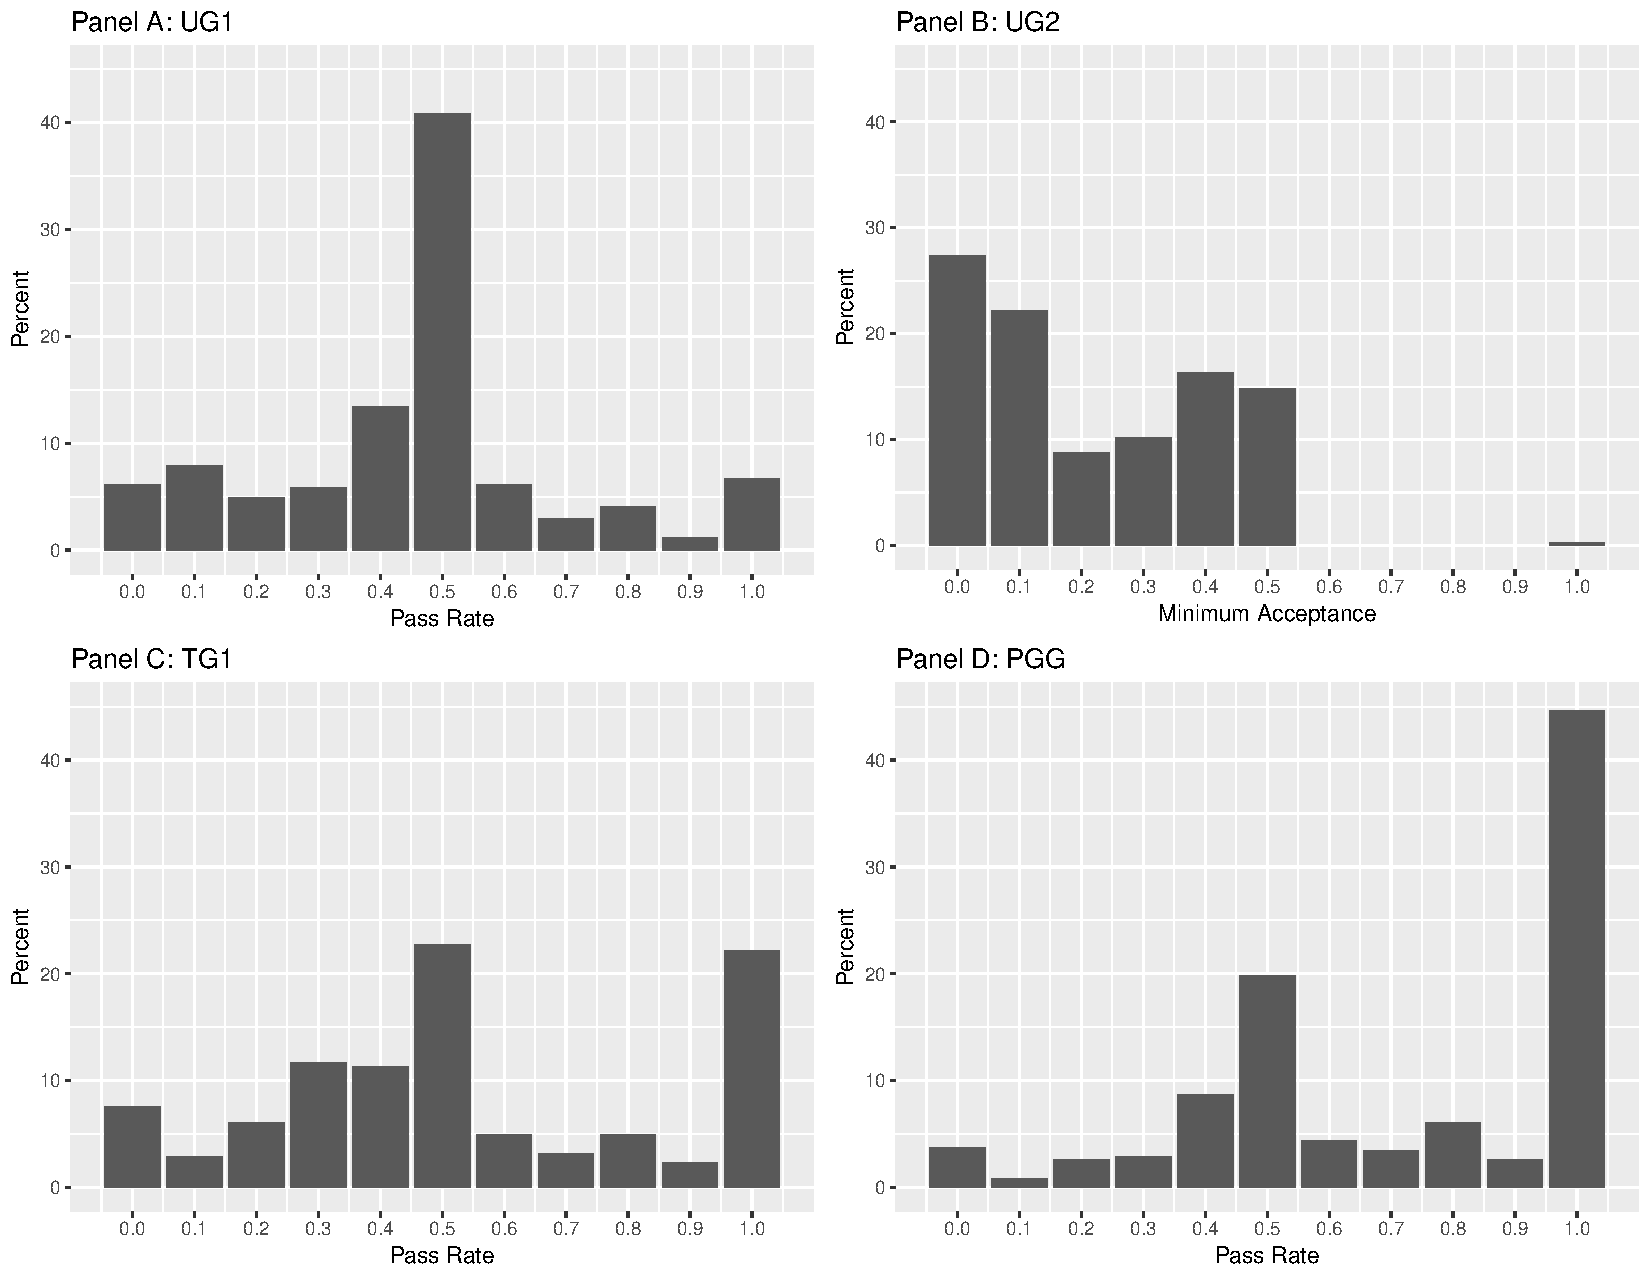
\includegraphics[scale=0.4]{Figure2a.pdf} \\



\noindent Figure 2: Distribution of responses in UG1, UG2, TG1, and PGG \\ \\
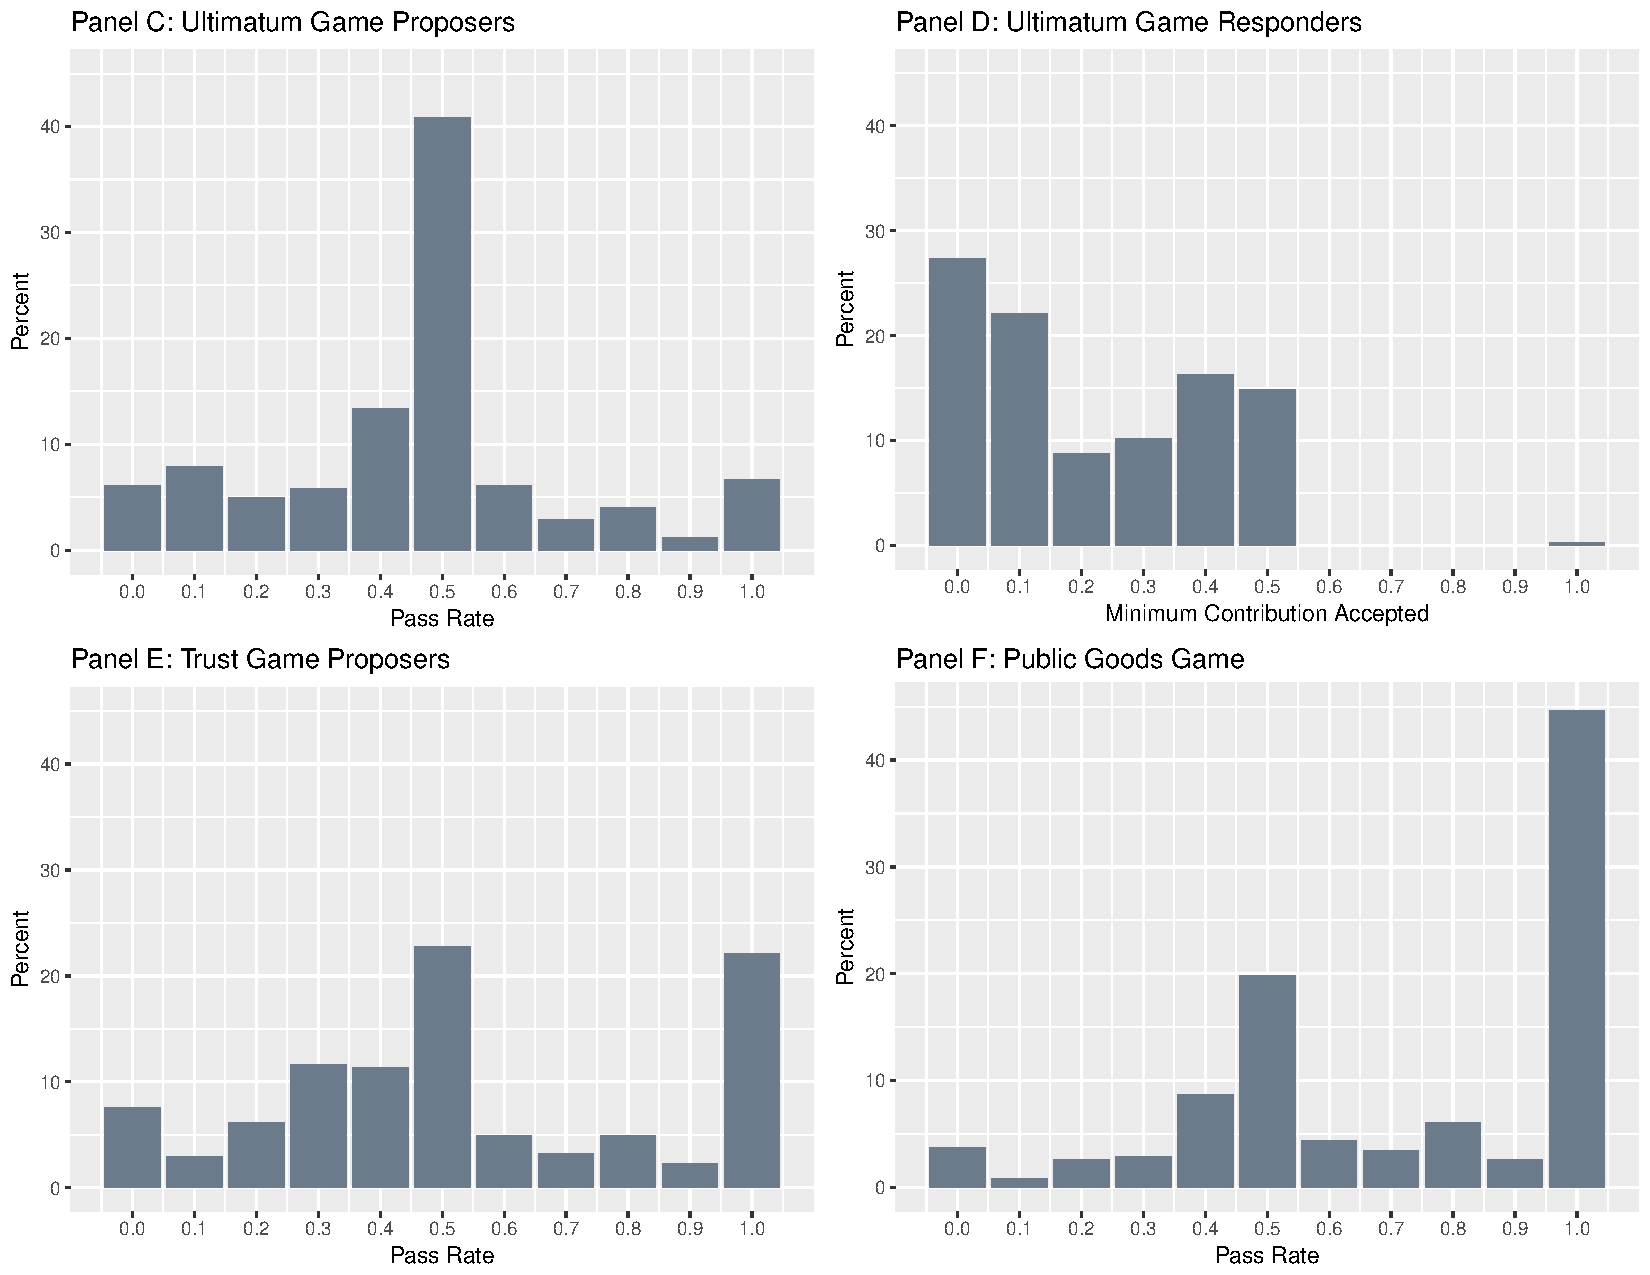
\includegraphics[scale=0.4]{Figure2b.pdf} \\

\noindent Figure 3: Distribution of responses from TG2 \\ \\
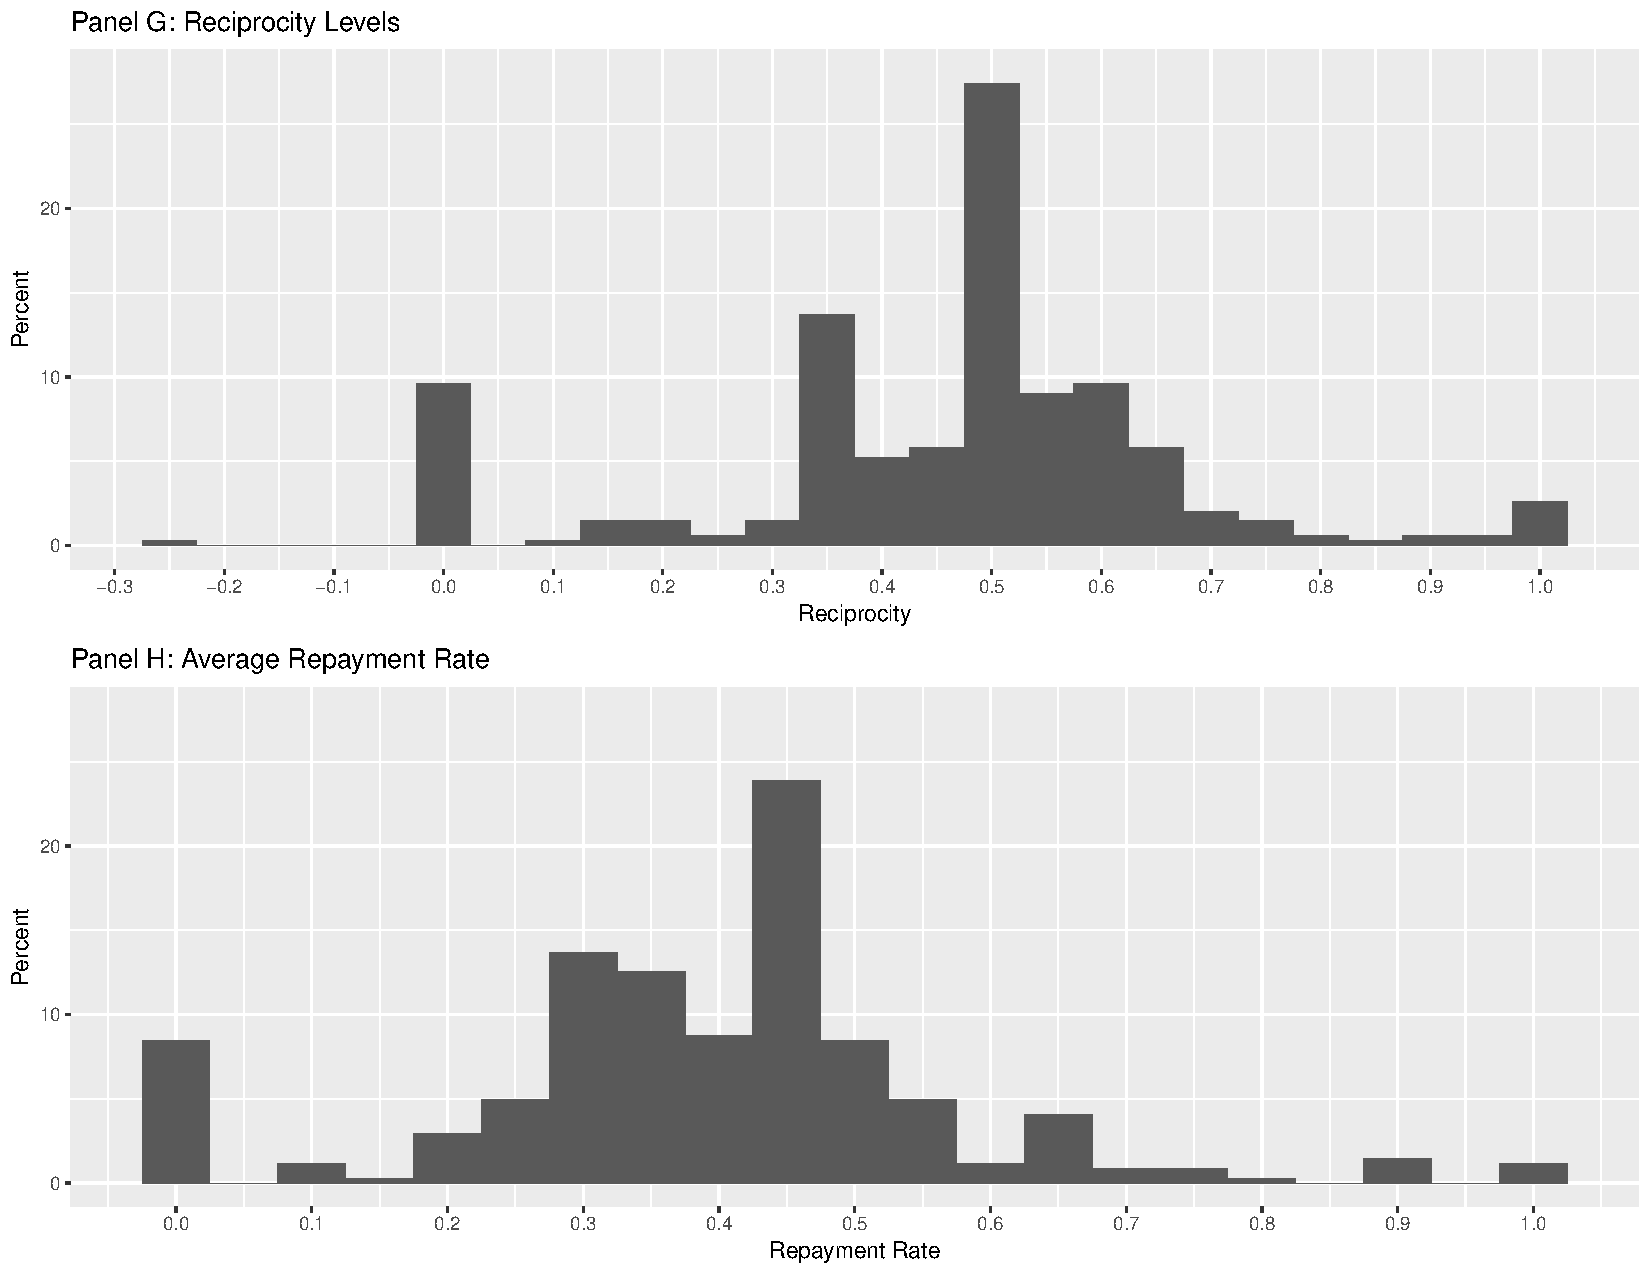
\includegraphics[scale=0.4]{Figure2c.pdf} \\



\noindent Figure 4: Total SRA scores\\ \\
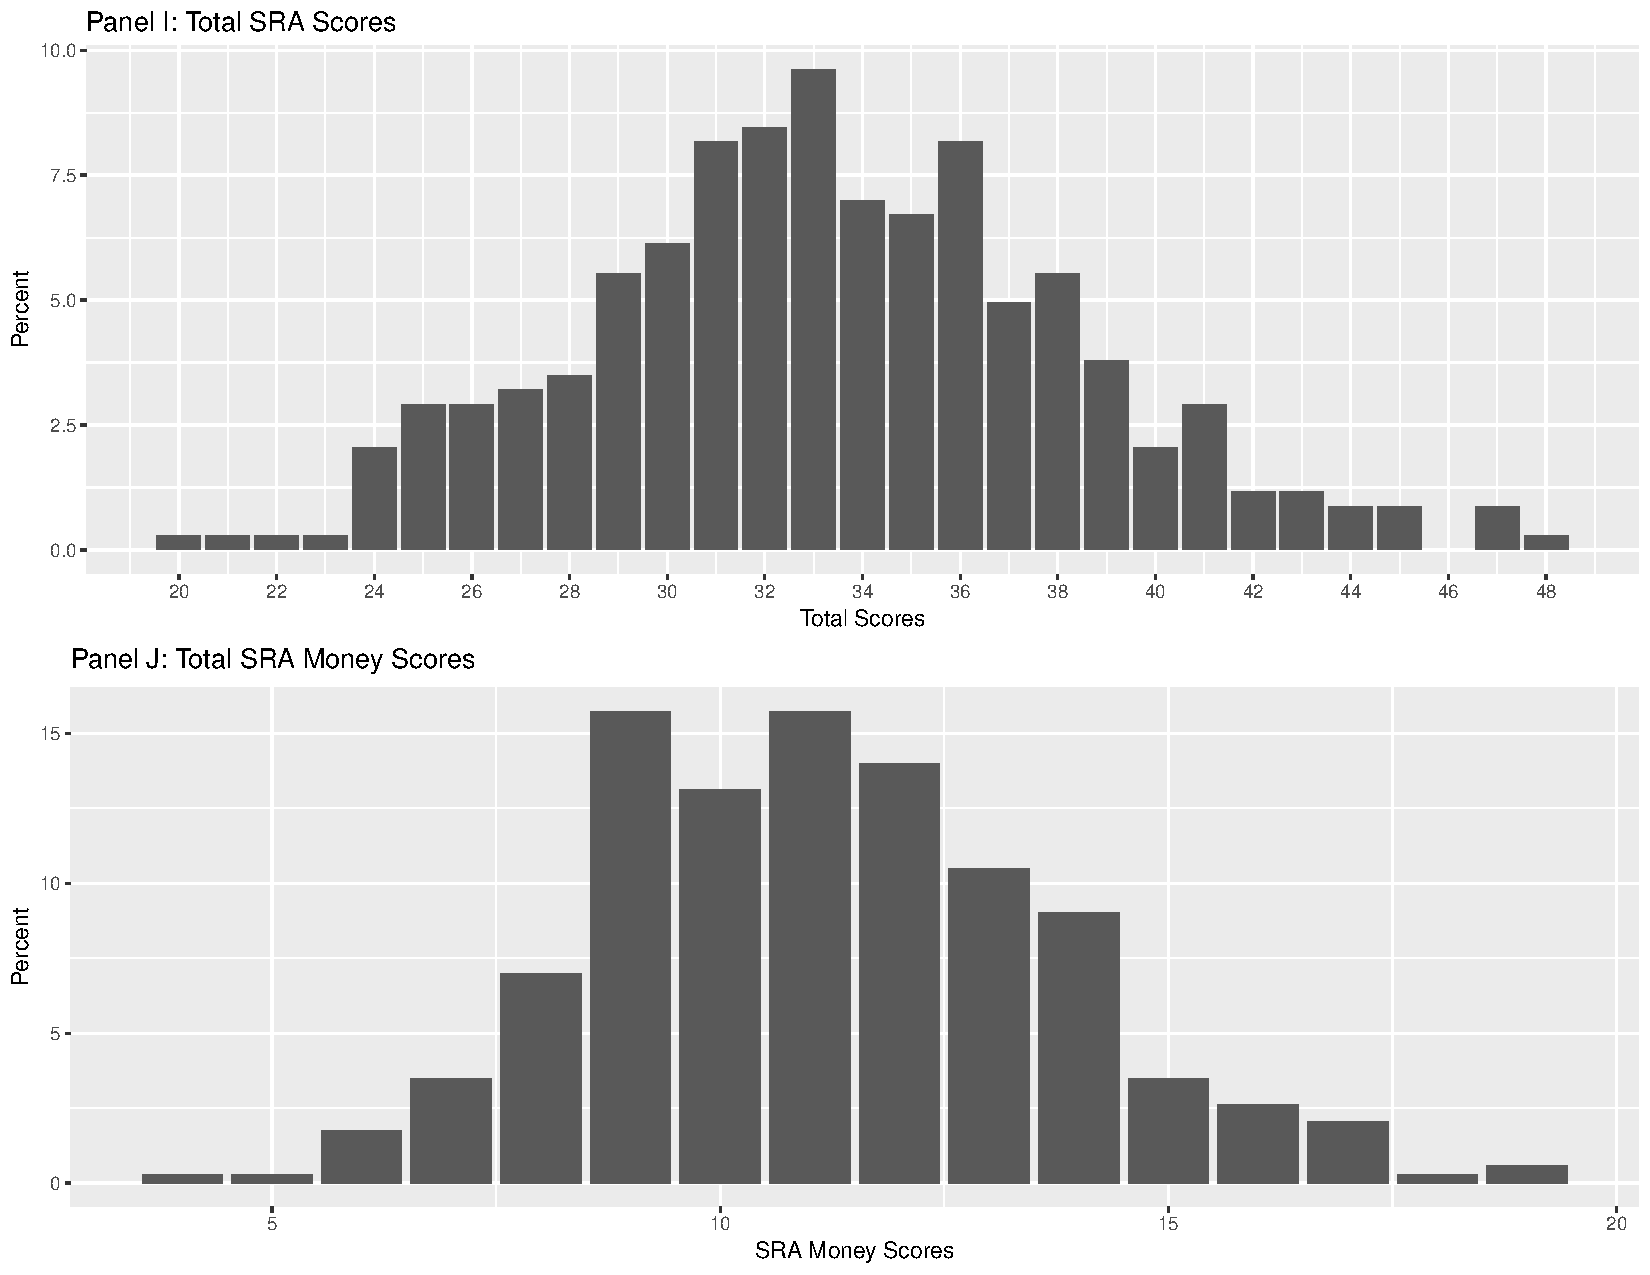
\includegraphics[scale=0.4]{Figure3.pdf}\\

\noindent Figure 5: Donations\\ \\
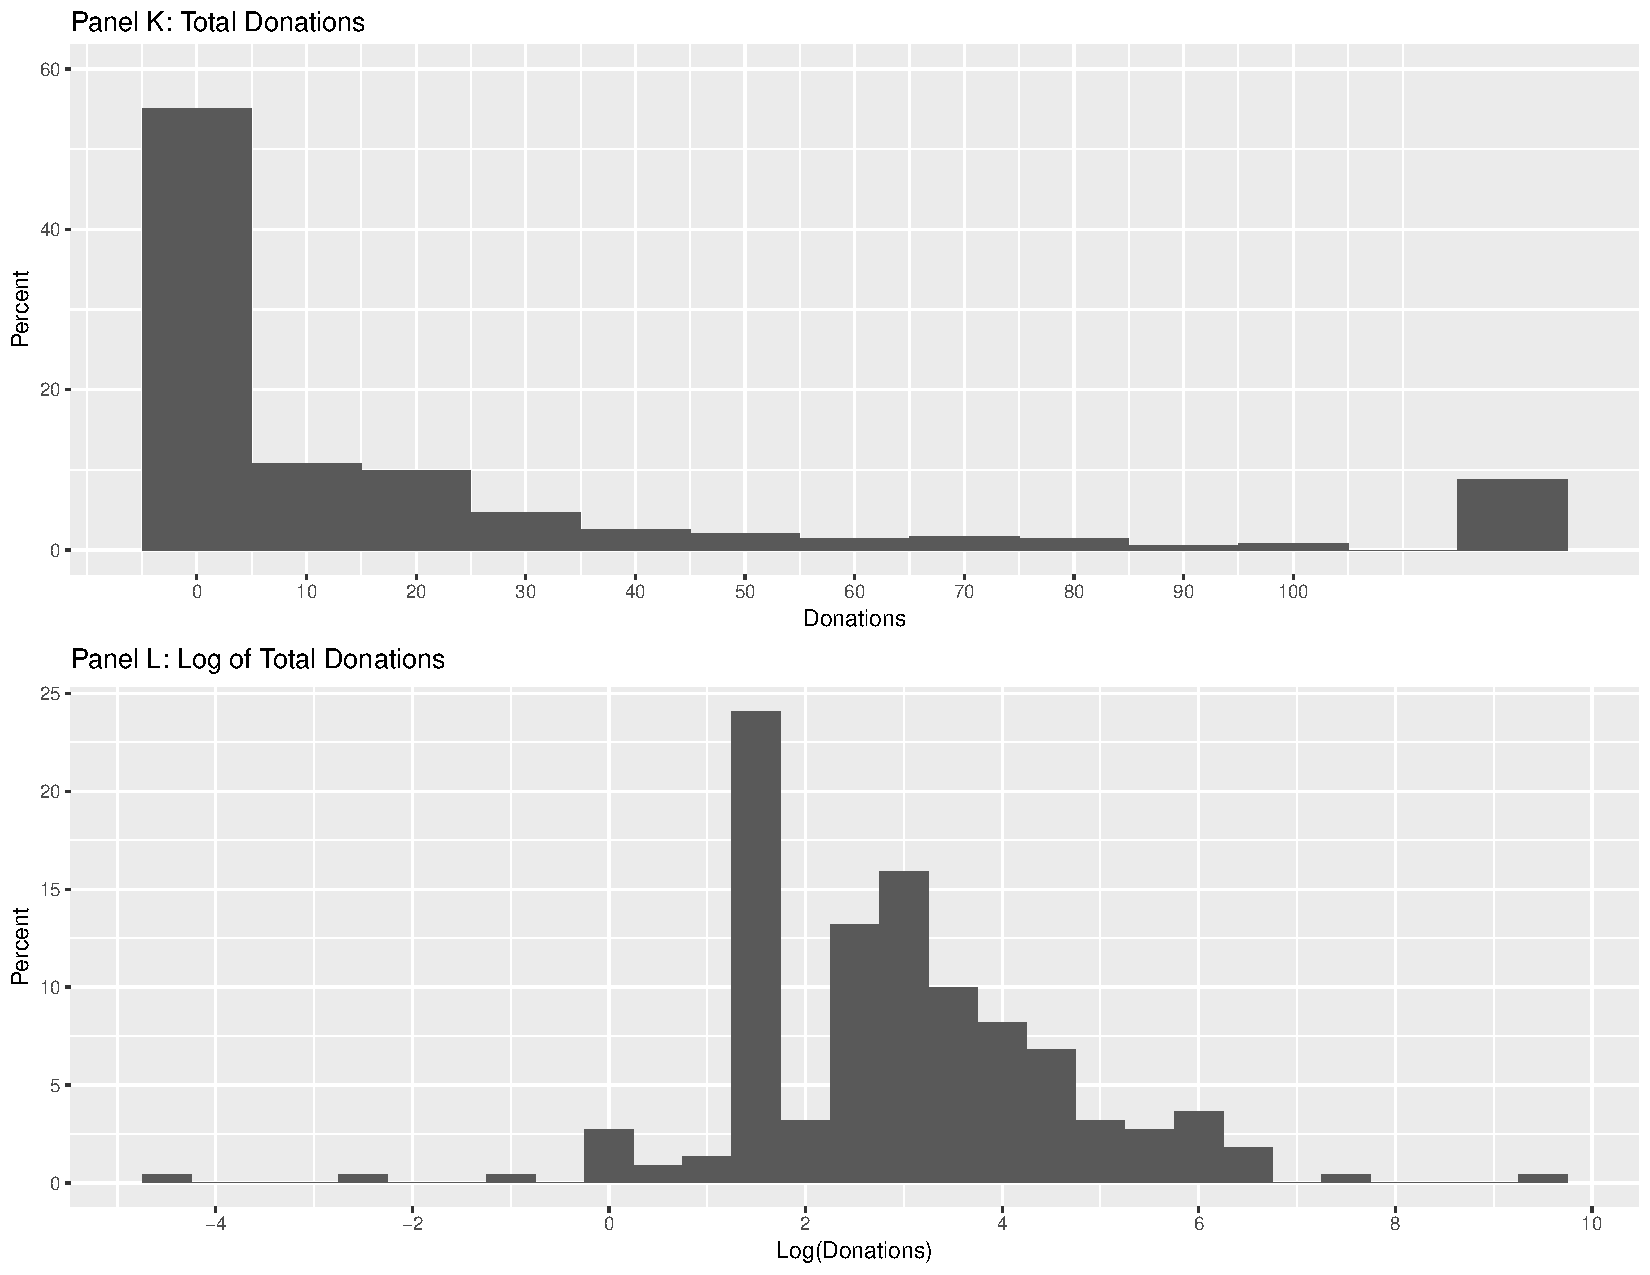
\includegraphics[scale=0.4]{Figure4.pdf}\\ \\



\begin{table}[!htbp] \centering 
  \caption{Pairwise correlations between game results (Spearman\rq s \(\rho\))} 
  \label{} \centering
  \begin{tabular}{rllllll}
  \hline
 & alpha &  \ UG1 & \ UG2 & \ TG1 & \ TG2 & \ PGG \\ 
  \hline
alpha &   \ 1.00  & -0.28*** & \ 0.04  & -0.26*** & -0.30*** & -0.16*** \\ 
  UG1 & -0.28*** & \ 1.00  &  \ 0.09  & \ 0.41*** & \ 0.31*** &  \ 0.30*** \\ 
  UG2 &  \ 0.04  &  \ 0.09  &  1.00  & -0.10* & -0.08  & -0.16*** \\ 
  TG1 & -0.26*** & \  0.41*** & -0.10* & \ 1.00  & \ 0.45*** &  \ 0.44*** \\ 
  TG2 & -0.30*** &  \ 0.31*** & -0.08  &  \ 0.45*** & \ 1.00  &  \ 0.21*** \\ 
  PGG & -0.16*** &  \ 0.30*** & -0.16*** & \  0.44*** & \ 0.21*** &  \ 1.00  \\ 
   \hline
      \textit{Note:}  & \multicolumn{6}{r}{$^{*}$p$<$0.1; $^{**}$p$<$0.05; $^{***}$p$<$0.01} \\ 
\end{tabular}
%\begin{tablenotes}\footnotesize
%\item Notes: 
%\item *, **,  and *** stand for statistical significance at the 10\%, 5\%, and 1\% levels.
%\item Alpha stands for \(\alpha\) levels derived from the generalized dictator game.
%\item UG1 and UG2 stand for Player 1 and Player 2 in ultimatum game, respectively.
%\item TG1 stands for Player 1 in trust game. 
%\item TG2 represents reciprocity levels for Player 2 in trust game.
%\item PGG stands for public goods game.
%\end{tablenotes}
\end{table}

\begin{table}[!htbp] \centering 
  \caption{Correlations between game results and SRA scores (Spearman\rq s \(\rho\))} 
  \label{} 
\centering
\begin{tabular}{rllllllll}
  \hline
 & SRAtotal & SRAmoney \\ 
  \hline
alpha  & -0.01  & \ \ -0.04  \\ 
  UG1  &  \ 0.02  &  \ \ \ 0.07  \\ 
  UG2 & -0.05  & \ \ -0.05  \\ 
  TG1 &  \ 0.07  &  \ \ \ 0.08  \\ 
  TG2  &  \ 0.04  & \ \ \  0.11** \\ 
  PGG  & \  0.06  &  \ \ \ 0.10* \\ 
  SRAtotal &  \ 1.00  &  \ \ \ 0.81*** \\ 
  SRAmoney  &  \ 0.81*** &  \ \ \ 1.00  \\ 
   \hline
   \textit{Note:}  & \multicolumn{2}{r}{$^{*}$p$<$0.1; $^{**}$p$<$0.05; $^{***}$p$<$0.01} \\ 
\end{tabular}
%\begin{tablenotes}\footnotesize
%\item Notes: 
%\item *, **,  and *** stand for statistical significance at the 10\%, 5\%, and 1\% levels.
%\item Alpha stands for \(\alpha\) levels derived from the generalized dictator game.
%\item UG1 and UG2 stand for Player 1 and Player 2 in ultimatum game, respectively.
%\item TG1 stands for Player 1 in trust game. 
%\item TG2 represents reciprocity levels for Player 2 in trust game.
%\item PGG stands for public goods game.
%\item SRAtotal stands for the total Self-Report Altruism score, and SRAmoney for those including only items related to money.
%\end{tablenotes}
\end{table}


\begin{table}[!htbp] \centering 
  \caption{Logistic regression models} 
  \label{} 
              \begin{adjustbox}{width=\textwidth}
\begin{tabular}{@{\extracolsep{5pt}}lcccccccccc} 
\\[-1.8ex]\hline 
\hline \\[-1.8ex] 
 & \multicolumn{10}{c}{\textit{Dependent variable:}} \\ 
\cline{2-11} 
\\[-1.8ex] & \multicolumn{10}{c}{Donated} \\ 
\\[-1.8ex] & (1) & (2) & (3) & (4) & (5) & (6) & (7) & (8) & (9) & (10)\\ 
\hline \\[-1.8ex] 
 Alpha & 0.052 &  &  &  &  &  &  &  & 0.064 & 0.065 \\ 
  & (0.086) &  &  &  &  &  &  &  & (0.093) & (0.093) \\ 
  & & & & & & & & & & \\ 
 UG1 &  & 0.016 &  &  &  &  &  &  & 0.002 & $-$0.005 \\ 
  &  & (0.107) &  &  &  &  &  &  & (0.125) & (0.125) \\ 
  & & & & & & & & & & \\ 
 UG2 &  &  & 0.120 &  &  &  &  &  & 0.136 & 0.138 \\ 
  &  &  & (0.137) &  &  &  &  &  & (0.142) & (0.142) \\ 
  & & & & & & & & & & \\ 
 TG1 &  &  &  & 0.011 &  &  &  &  & $-$0.001 & 0.006 \\ 
  &  &  &  & (0.083) &  &  &  &  & (0.105) & (0.105) \\ 
  & & & & & & & & & & \\ 
 Reciprocity &  &  &  &  & 0.025 &  &  &  & 0.045 & 0.031 \\ 
  &  &  &  &  & (0.120) &  &  &  & (0.140) & (0.140) \\ 
  & & & & & & & & & & \\ 
 PGG &  &  &  &  &  & 0.024 &  &  & 0.034 & 0.028 \\ 
  &  &  &  &  &  & (0.086) &  &  & (0.099) & (0.099) \\ 
  & & & & & & & & & & \\ 
 SRAtotal &  &  &  &  &  &  & 0.007 &  & 0.007 &  \\ 
  &  &  &  &  &  &  & (0.005) &  & (0.005) &  \\ 
  & & & & & & & & & & \\ 
 SRAmoney &  &  &  &  &  &  &  & 0.016 &  & 0.016 \\ 
  &  &  &  &  &  &  &  & (0.010) &  & (0.010) \\ 
  & & & & & & & & & & \\ 
 Constant & 0.614$^{***}$ & 0.634$^{***}$ & 0.616$^{***}$ & 0.635$^{***}$ & 0.630$^{***}$ & 0.624$^{***}$ & 0.400$^{**}$ & 0.461$^{***}$ & 0.291 & 0.360$^{**}$ \\ 
  & (0.052) & (0.056) & (0.039) & (0.052) & (0.061) & (0.067) & (0.176) & (0.117) & (0.208) & (0.158) \\ 
  & & & & & & & & & & \\ 
\hline \\[-1.8ex] 
Observations & 343 & 343 & 343 & 343 & 343 & 343 & 343 & 343 & 343 & 343 \\ 
Log Likelihood & $-$235.468 & $-$235.640 & $-$235.264 & $-$235.642 & $-$235.629 & $-$235.611 & $-$234.689 & $-$234.392 & $-$233.916 & $-$233.620 \\ 
Akaike Inf. Crit. & 474.937 & 475.280 & 474.528 & 475.284 & 475.258 & 475.222 & 473.378 & 472.785 & 483.831 & 483.239 \\ 
Pseudo-R$^{2}$ & 0.000778 & 0.000048 & 0.001649 & 0.000039 & 0.000095 & 0.000172 & 0.00410 & 0.005364 & 0.007396 & 0.008658\\
\hline 
\hline \\[-1.8ex] 
\textit{Note:}  & \multicolumn{10}{r}{$^{*}$p$<$0.1; $^{**}$p$<$0.05; $^{***}$p$<$0.01} \\ 
\end{tabular} 
%\textit{Note:}  *, **,  and *** represent statistical significance at the 10\%, 5\%, and 1\% levels, respectively. \\ Alpha stands for \(\alpha\) levels derived from the generalized dictator game. \\ UG1 and UG2 stand for Player 1 and Player 2 in ultimatum game, respectively. \\ TG1 stands for Player 1 in trust game. \\ TG2 represents reciprocity levels for Player 2 in trust game. \\ PGG stands for public goods game. \\ SRAtotal stands for the total Self-Report Altruism score, and SRAmoney for those including only items related to money. \\
\end{adjustbox}
%\begin{tablenotes}\footnotesize
%\item Notes: 
%\item *, **,  and *** stand for statistical significance at the 10\%, 5\%, and 1\% levels.
%\item Alpha stands for \(\alpha\) levels derived from the generalized dictator game.
%\item UG1 and UG2 stand for Player 1 and Player 2 in ultimatum game, respectively.
%\item TG1 stands for Player 1 in trust game. 
%\item TG2 represents reciprocity levels for Player 2 in trust game.
%\item PGG stands for public goods game.
%\item SRAtotal stands for the total Self-Report Altruism score, and SRAmoney for those including only items related to money.
%\end{tablenotes}
\end{table} 




\begin{table}[!htbp] \centering 
  \caption{Tobit regression models} 
  \label{} 
            \begin{adjustbox}{width=\textwidth}
\begin{tabular}{@{\extracolsep{5pt}}lcccccccccc} 
\\[-1.8ex]\hline 
\hline \\[-1.8ex] 
 & \multicolumn{10}{c}{\textit{Dependent variable:}} \\ 
\cline{2-11} 
\\[-1.8ex] & \multicolumn{10}{c}{Donations} \\ 
\\[-1.8ex] & (1) & (2) & (3) & (4) & (5) & (6) & (7) & (8) & (9) & (10)\\ 
\hline \\[-1.8ex] 
 Alpha & 3.31909 &  &  &  &  &  &  &  & 3.65579 & 3.84605 \\ 
  & (7.74063) &  &  &  &  &  &  &  & (7.12276) & (7.08913) \\ 
  & & & & & & & & & & \\ 
 UG1 &  & 6.86161 &  &  &  &  &  &  & 7.83768 & 7.02630 \\ 
  &  & (8.35099) &  &  &  &  &  &  & (9.46080) & (9.41465) \\ 
  & & & & & & & & & & \\ 
 UG2 &  &  & 6.02451 &  &  &  &  &  & 7.15663 & 7.38378 \\ 
  &  &  & (10.74423) &  &  &  &  &  & (10.91164) & (10.85998) \\ 
  & & & & & & & & & & \\ 
 TG1 &  &  &  & 0.40224 &  &  &  &  & $-$3.11720 & $-$2.26672 \\ 
  &  &  &  & (6.48083) &  &  &  &  & (8.11155) & (8.05751) \\ 
  & & & & & & & & & & \\ 
 TG2 &  &  &  &  & $-$7.78095 &  &  &  & $-$10.19879 & $-$11.88385 \\ 
  &  &  &  &  & (9.33936) &  &  &  & (10.64798) & (10.63425) \\ 
  & & & & & & & & & & \\ 
 PGG &  &  &  &  &  & 9.74202 &  &  & 11.30993 & 10.36290 \\ 
  &  &  &  &  &  & (6.73445) &  &  & (7.57870) & (7.55598) \\ 
  & & & & & & & & & & \\ 
 SRAtotal &  &  &  &  &  &  & 0.70389$^{*}$ &  & 0.71276$^{*}$ &  \\ 
  &  &  &  &  &  &  & (0.40552) &  & (0.40407) &  \\ 
  & & & & & & & & & & \\ 
 SRAmoney &  &  &  &  &  &  &  & 1.95175$^{**}$ &  & 1.96099$^{**}$ \\ 
  &  &  &  &  &  &  &  & (0.79090) &  & (0.79215) \\ 
  & & & & & & & & & & \\ 
 Constant & 7.12277$^{*}$ & 5.71272 & 7.56796$^{**}$ & 8.63908$^{**}$ & 12.43205$^{***}$ & 1.89668 & $-$14.61146 & $-$12.89298 & $-$23.64445 & $-$20.51751$^{*}$ \\ 
  & (4.10025) & (4.37273) & (3.10718) & (4.09095) & (4.73771) & (5.27791) & (13.73187) & (9.12441) & (16.08117) & (12.25384) \\ 
  & & & & & & & & & & \\ 
\hline \\[-1.8ex] 
Observations & 343 & 343 & 343 & 343 & 343 & 343 & 343 & 343 & 343 & 343 \\ 
Pseudo-R$^{2}$ & 0.000124 & 0.000346 & 0.000161 & 0.000002 & 0.000356 & 0.001073 & 0.001548 & 0.003140 & 0.004026 & 0.005588\\
\hline 
\hline \\[-1.8ex] 
\textit{Note:}  & \multicolumn{10}{r}{$^{*}$p$<$0.1; $^{**}$p$<$0.05; $^{***}$p$<$0.01} \\ 
\end{tabular} 
\end{adjustbox}
\end{table} 





\begin{table}[!htbp] \centering 
  \caption{Best-subset logistic regression} 
  \label{} 
\begin{tabular}{@{\extracolsep{5pt}}lc} 
\\[-1.8ex]\hline 
\hline \\[-1.8ex] 
 & \multicolumn{1}{c}{\textit{Dependent variable:}} \\ 
\cline{2-2} 
\\[-1.8ex] & Donated \\ 
\hline \\[-1.8ex] 
 SRA3 & $-$0.096$^{***}$ \\ 
  & (0.028) \\ 
  & \\ 
 SRA4 & 0.123$^{***}$ \\ 
  & (0.030) \\ 
  & \\ 
 SRA8 & 0.075$^{**}$ \\ 
  & (0.034) \\ 
  & \\ 
 SRA10 & $-$0.052$^{**}$ \\ 
  & (0.025) \\ 
  & \\ 
 Constant & 0.386$^{**}$ \\ 
  & (0.155) \\ 
  & \\ 
\hline \\[-1.8ex] 
Observations & 343 \\ 
Log Likelihood & $-$220.385 \\ 
Akaike Inf. Crit. & 450.770 \\ 
Psuedo-R$^{2}$ & 0.06506 \\
\hline 
\hline \\[-1.8ex] 
\textit{Note:}  & \multicolumn{1}{r}{$^{*}$p$<$0.1; $^{**}$p$<$0.05; $^{***}$p$<$0.01} \\ 
\end{tabular} 
\end{table} 


\begin{table}[!htbp] \centering 
  \caption{Best-subset tobit regression} 
  \label{} 
\begin{tabular}{@{\extracolsep{5pt}}lc} 
\\[-1.8ex]\hline 
\hline \\[-1.8ex] 
 & \multicolumn{1}{c}{\textit{Dependent variable:}} \\ 
\cline{2-2} 
\\[-1.8ex] & Donations \\ 
\hline \\[-1.8ex] 
 Rho & $-$0.0004592 \\ 
  & (0.0005748) \\ 
  & \\ 
 Constant & 8.21167$^{***}$ \\ 
  & (2.22776) \\ 
  & \\ 
\hline \\[-1.8ex] 
Observations & 343 \\ 
Psuedo-R$^{2}$ & 0.000325 \\
\hline 
\hline \\[-1.8ex] 
\textit{Note:}  & \multicolumn{1}{r}{$^{*}$p$<$0.1; $^{**}$p$<$0.05; $^{***}$p$<$0.01} \\ 
\end{tabular} 
\end{table} 





\begin{table}[!htbp] \centering 
  \caption{Lasso penalized logistic model} 
  \label{} 
\begin{tabular}{@{\extracolsep{5pt}}lc} 
\\[-1.8ex]\hline 
\hline \\[-1.8ex] 
 & \multicolumn{1}{c}{\textit{Dependent variable:}} \\ 
\cline{2-2} 
\\[-1.8ex] & Donated \\ 
\hline \\[-1.8ex] 

 SRA3 & $-$0.00680$^{**}$ \\ 
  & \\ 
 SRA4 & 0.14486$^{**}$ \\ 
  & \\ 
  Constant & 0.12090 \\ 
  & \\ 
\hline \\[-1.8ex] 

\hline \\[-1.8ex] 
\textit{Note:}  & \multicolumn{1}{r}{$^{*}$p$<$0.1; $^{**}$p$<$0.05; $^{***}$p$<$0.01} \\ 
\end{tabular} 
\end{table} 



\end{document}